% Mini research note on recovery, honest-grid validation, and saddle diagnostics.
\documentclass[11pt]{article}
% Shared preamble for the research-note series.
% Create note-specific content in the per-note directory; keep common macros here.
\usepackage[margin=1in]{geometry}
\usepackage[T1]{fontenc}
\usepackage[utf8]{inputenc}
\usepackage{amsmath,amssymb}
\usepackage{booktabs,longtable,array}
\usepackage{graphicx}
\usepackage{float}
\usepackage{enumitem}
\usepackage{xcolor}
\usepackage{hyperref}
\usepackage{caption}
\usepackage{titlesec}
\hypersetup{colorlinks=true, linkcolor=blue!60!black, urlcolor=blue!60!black, citecolor=blue!60!black}
\setlist[itemize]{leftmargin=1.25em, itemsep=0.2em, topsep=0.3em}
\setlist[enumerate]{leftmargin=1.4em, itemsep=0.2em, topsep=0.3em}
\setlength{\parindent}{0pt}
\setlength{\parskip}{0.6em}
\newcommand{\statusbox}[2]{%
  \noindent\fcolorbox{black}{gray!10}{%
    \parbox{\dimexpr\linewidth-2\fboxsep-2\fboxrule\relax}{%
      \textbf{Status:} #1\\#2
    }%
  }
}

% Shared notation helpers for the research-note series.
\newcommand{\Jlin}{J}
\newcommand{\Jphys}{J_{\mathrm{phys}}}
\newcommand{\Jsurf}{J_{\mathrm{surf}}}
\newcommand{\JdB}{J_{\mathrm{dB}}}
\newcommand{\phiopt}{\phi_{\mathrm{opt}}}
\newcommand{\sigmathreedb}{\sigma_{3\mathrm{dB}}}
\newcommand{\Nt}{N_t}
\newcommand{\Nphi}{N_{\phi}}
\newcommand{\Lfiber}{L}
\newcommand{\Pcont}{P}
\newcommand{\band}{\mathcal{B}_{\mathrm{Raman}}}
\newcommand{\todoitem}[1]{\textcolor{red!70!black}{\textbf{TODO:} #1}}


\title{Recovery, Honest Grids, and Saddle Diagnostics}
\author{Fiber Raman Suppression Project}
\date{Evidence snapshot: 2026-04-26}

\begin{document}
\maketitle

\begin{abstract}
This note explains the project lane that checks whether strong Raman
suppression results survive stricter numerical validation, and what the
remaining local geometry says about optimization. The main lesson is that
recovery is not just re-running an optimizer: a result only counts if the pulse
fits inside the simulated time window, energy drift is small, the same phase
state can be found or revalidated, and the standard diagnostic images look
physically sane. On that standard, several single-mode anchors survive, one
simple-profile sweep is retired, and the high-performing branch remains
saddle-like rather than minimum-like. The practical conclusion is that future
optimizers should combine honest-grid validation, basis continuation, and
explicit negative-curvature handling.
\end{abstract}

\section*{Claim Status}
\statusbox{established with scoped limits}{The honest-grid recovery evidence is
strong for the single-mode anchors shown in this note. The saddle evidence is
strong for the canonical SMF-28 control ladder, but should not be overclaimed
as a theorem for every fiber, power, or multimode setting. The retired sweep
result is also important: not every visually impressive or deep result survives
the boundary check.}

\section{Question and Thesis}

The question is simple: when a saved optimization result looks good, how do we
know it is a real Raman-suppression result and not a simulation artifact?

The thesis is that a result should pass three separate tests:
\begin{enumerate}
    \item \textbf{physics test:} the output pulse stays inside the simulated
    time window instead of touching the edges;
    \item \textbf{optimization test:} the reported objective still holds after
    revalidation or re-optimization on the repaired grid;
    \item \textbf{geometry test:} if the optimizer stops, the local Hessian
    tells us whether the point is minimum-like or saddle-like.
\end{enumerate}

Those tests change the story in a useful way. Some results become more
credible. Some become weaker lower bounds. Some are retired. The saddle
diagnostics also explain why first-order L-BFGS can stop at points that are
useful but not true local minima.

\subsection*{Intuition Check}

The easy mistake is to trust a small dB number by itself. A small number is not
enough. The pulse also has to stay away from the time-window boundary, because
otherwise the optimizer may be exploiting the numerical box instead of the
fiber physics.

\section{The Numerical Failure Mode}

The forward model propagates a shaped input spectrum
\[
    u_\omega(0;\phi)=u_{\omega,0}e^{i\phi(\omega)}
\]
through a nonlinear fiber model and measures the output Raman-band energy
fraction,
\[
    \Jphys(\phi)
    =
    \frac{\sum_{\omega_k\in\band}|u_{\omega_k}(L;\phi)|^2}
         {\sum_k |u_{\omega_k}(L;\phi)|^2}.
\]
The reported value is
\[
    \JdB(\phi)=10\log_{10}\Jphys(\phi).
\]

This objective is only meaningful if the numerical grid is large enough. The
time window has finite edges. If nonlinear broadening, dispersion, or an
arbitrary group delay pushes the pulse into those edges, the FFT-periodic
solver can wrap or contaminate the output. The recovery lane therefore measures
an edge fraction,
\[
    \eta_{\mathrm{edge}}
    =
    \frac{\int_{\mathrm{edge}} |u(t,L)|^2\,dt}
         {\int_{\mathrm{all}} |u(t,L)|^2\,dt},
\]
where the edge region is the beginning and end of the simulated time window.
The working acceptance rule is
\[
    \eta_{\mathrm{edge}} < 10^{-3}.
\]

Energy drift is checked separately:
\[
    \delta_E
    =
    \frac{\left|E_{\mathrm{out}}-E_{\mathrm{in}}\right|}
         {\max(E_{\mathrm{in}},\epsilon)}.
\]
Low edge fraction checks boundary containment. Low energy drift checks that the
propagator is not quietly losing or gaining too much energy.

\subsection*{Intuition Check}

The edge check is like making sure a photograph did not crop off part of the
object. If the pulse hits the edge of the time window, the optimizer may still
report a nice number, but we no longer know whether that number came from real
fiber dynamics.

\section{Honest-Grid Recovery Method}

The recovery workflow starts from an existing candidate phase, repairs the
grid, and then decides whether the candidate survives.

\begin{figure}[H]
\centering
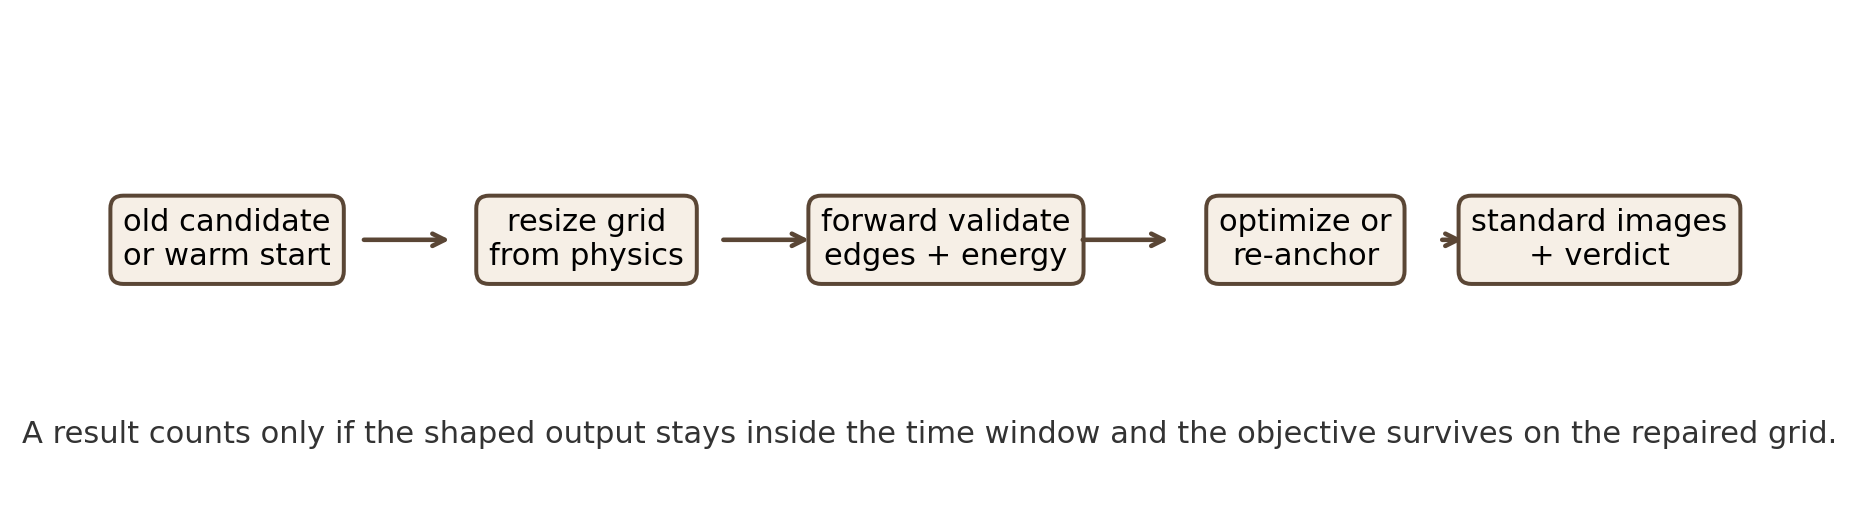
\includegraphics[width=0.96\linewidth]{figures/recovery_validation_workflow.png}
\caption{Honest-grid recovery loop. Old candidates are not accepted directly:
the grid is resized from physical estimates, the field is forward-validated,
optimization or re-anchoring is rerun when needed, and the final verdict is
based on scalar diagnostics plus standard images.}
\end{figure}

The grid choice is not arbitrary. The first guess comes from the expected
dispersive walk-off and nonlinear broadening. In words,
\[
    \text{window size}
    \approx
    \text{pulse width}
    + \text{dispersion walk-off}
    + \text{SPM-broadened safety margin}.
\]
The estimate only proposes a starting grid. The actual gate is empirical:
propagate the flat pulse and the relevant warm-started phase on the candidate
grid, then double the time window if the output edge fraction fails.

For a saved phase \(\phi_{\mathrm{old}}\), recovery also removes the two
obvious phase gauges before judging the grid:
\[
    \phi_{\mathrm{fixed}}(\omega)
    =
    \phi_{\mathrm{old}}(\omega)
    -
    (a+b\omega).
\]
The constant term is a global phase. The linear term is a time shift. Neither
changes the Raman-band fraction physically, but both can make a saved phase
look artificially wide in time if left in place.

\subsection*{Intuition Check}

Subtracting \(a+b\omega\) is not changing the real control in a meaningful way.
It is just choosing a cleaner coordinate system. A constant phase and a rigid
time shift are like moving the ruler, not changing the pulse physics.

\section{Result Verdicts}

\begin{figure}[H]
\centering
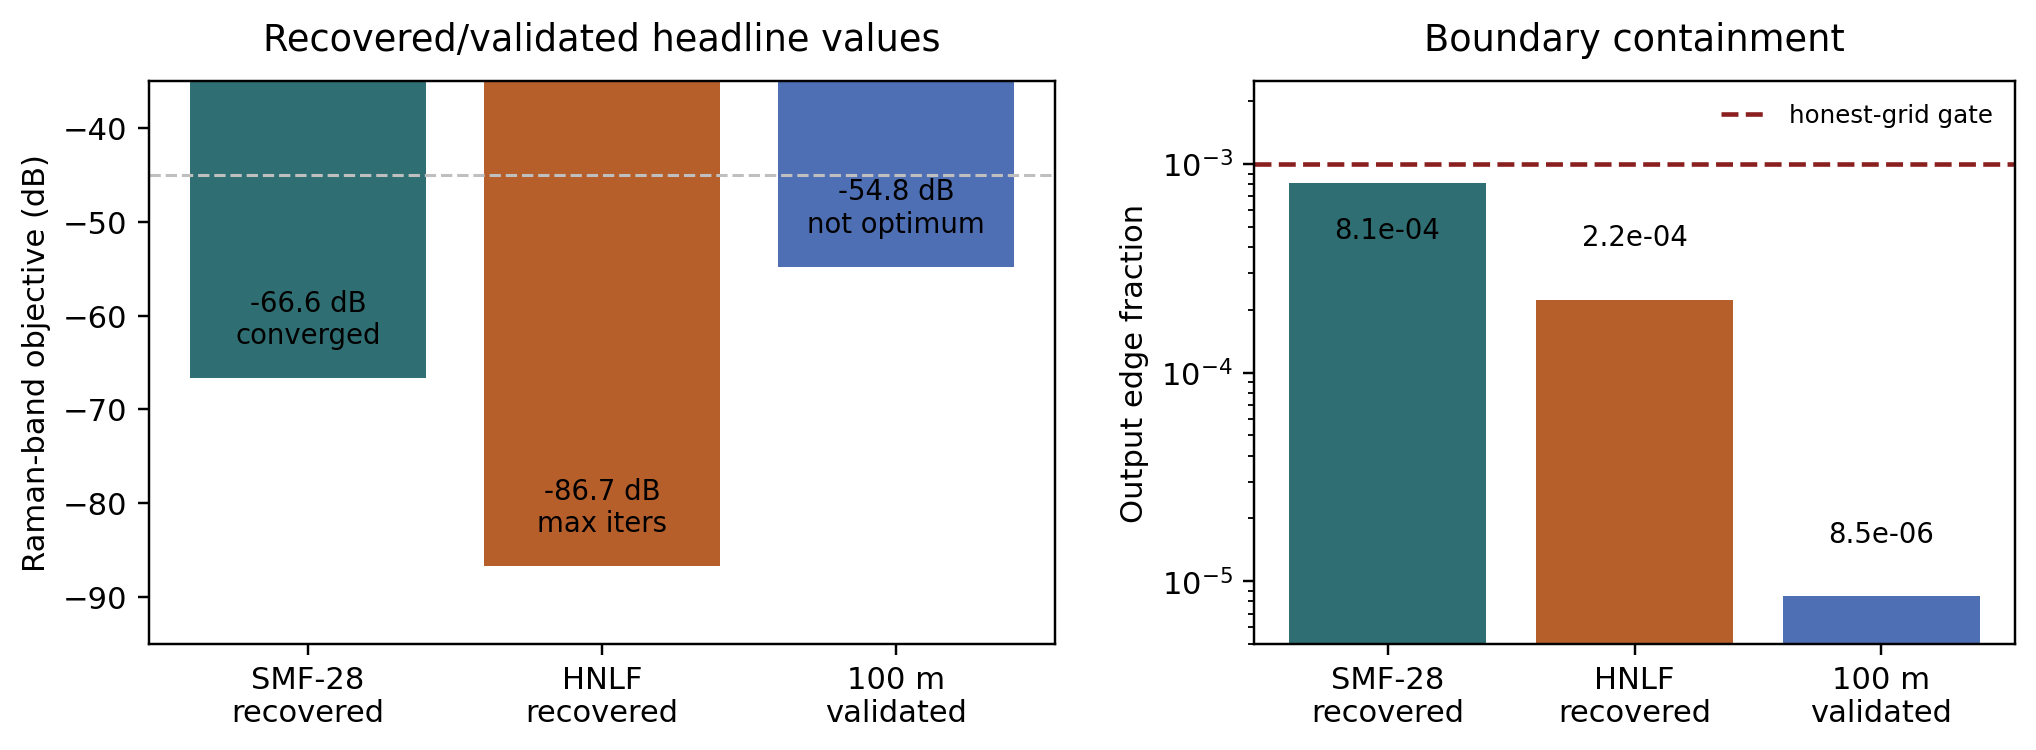
\includegraphics[width=0.92\linewidth]{figures/recovery_anchor_summary_clean.png}
\caption{Recovered and validated anchors. The dashed edge-fraction line marks
the \(10^{-3}\) acceptance gate. The HNLF and 100 m entries are useful but
should be described carefully because their stored optimizer flags did not
certify convergence.}
\end{figure}

\begin{center}
\small
\resizebox{\linewidth}{!}{%
\begin{tabular}{>{\raggedright\arraybackslash}p{0.22\linewidth}
                >{\raggedright\arraybackslash}p{0.24\linewidth}
                >{\raggedleft\arraybackslash}p{0.12\linewidth}
                >{\raggedleft\arraybackslash}p{0.13\linewidth}
                >{\raggedright\arraybackslash}p{0.28\linewidth}}
\toprule
\textbf{Case} & \textbf{Regime} & \textbf{Objective} & \textbf{Edge frac.} & \textbf{Verdict} \\
\midrule
Recovered SMF-28 anchor & \(L=2.0\,\mathrm{m}\), \(P=0.2\,\mathrm{W}\) &
\(-66.61\,\mathrm{dB}\) & \(8.10\times10^{-4}\) &
Recovered and converged on the repaired grid. \\
Recovered HNLF anchor & \(L=0.5\,\mathrm{m}\), \(P=0.01\,\mathrm{W}\) &
\(-86.68\,\mathrm{dB}\) & \(2.24\times10^{-4}\) &
Recovered, but the run stopped at the iteration cap. Treat as a strong achieved
value, not a proved optimum. \\
Validated long-fiber lower bound & \(L=100\,\mathrm{m}\), \(P=0.05\,\mathrm{W}\) &
\(-54.77\,\mathrm{dB}\) & \(8.47\times10^{-6}\) &
Revalidated from the full saved state. Honest lower bound, not a convergence
claim. \\
Retired simple-control sweep & \(L=2.0\,\mathrm{m}\), \(P=0.2\,\mathrm{W}\) &
best \(-66.03\,\mathrm{dB}\) & \(8.42\times10^{-2}\) &
Fails the boundary gate; do not use as a clean simplicity claim. \\
\bottomrule
\end{tabular}}
\end{center}

\subsection*{Intuition Check}

The table has two columns that matter most: objective and edge fraction. A deep
objective with a large edge fraction is not a clean win. A less dramatic result
that passes the edge gate can be more scientifically useful.

\clearpage
\section{Representative Result Pages}

Each page pairs the phase diagnostic with the corresponding spectral-evolution
heat map. The phase diagnostic says what input control was applied. The heat
map says how the spectrum evolved inside the fiber.

\begin{figure}[p]
\centering
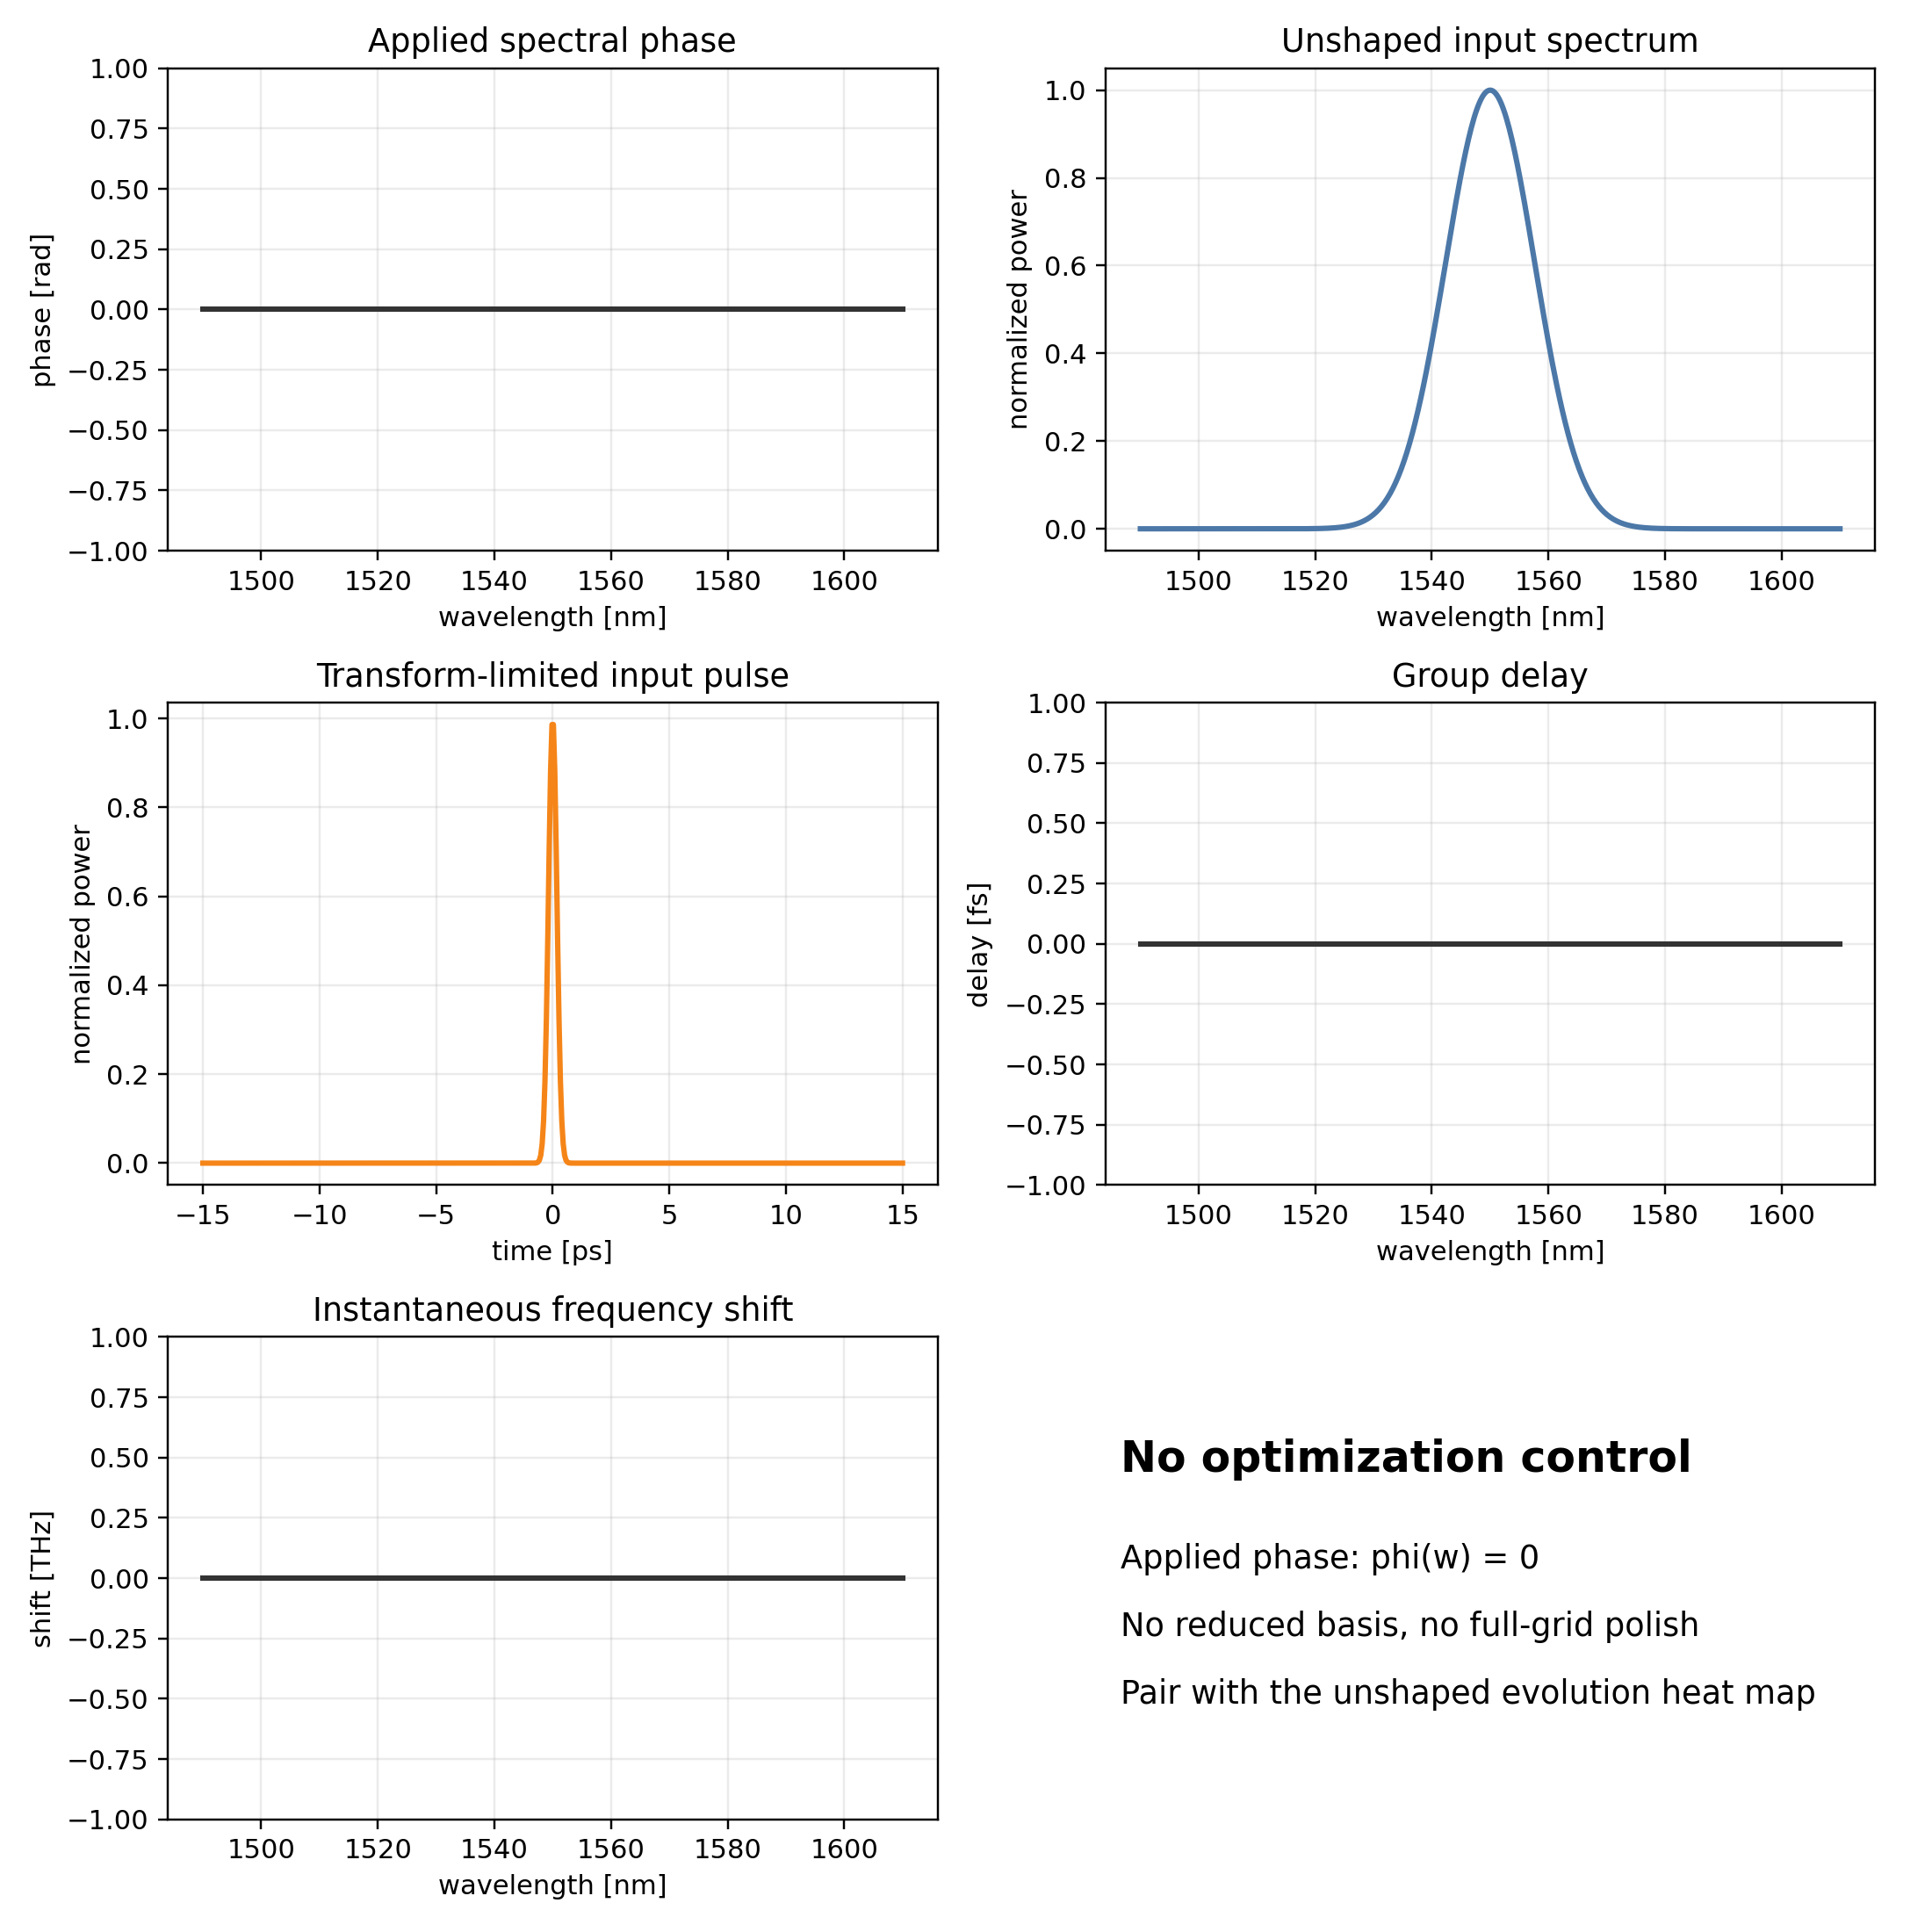
\includegraphics[height=0.47\textheight]{figures/control_smf28_no_shaping_phase_diagnostic.png}
\vspace{0.5em}

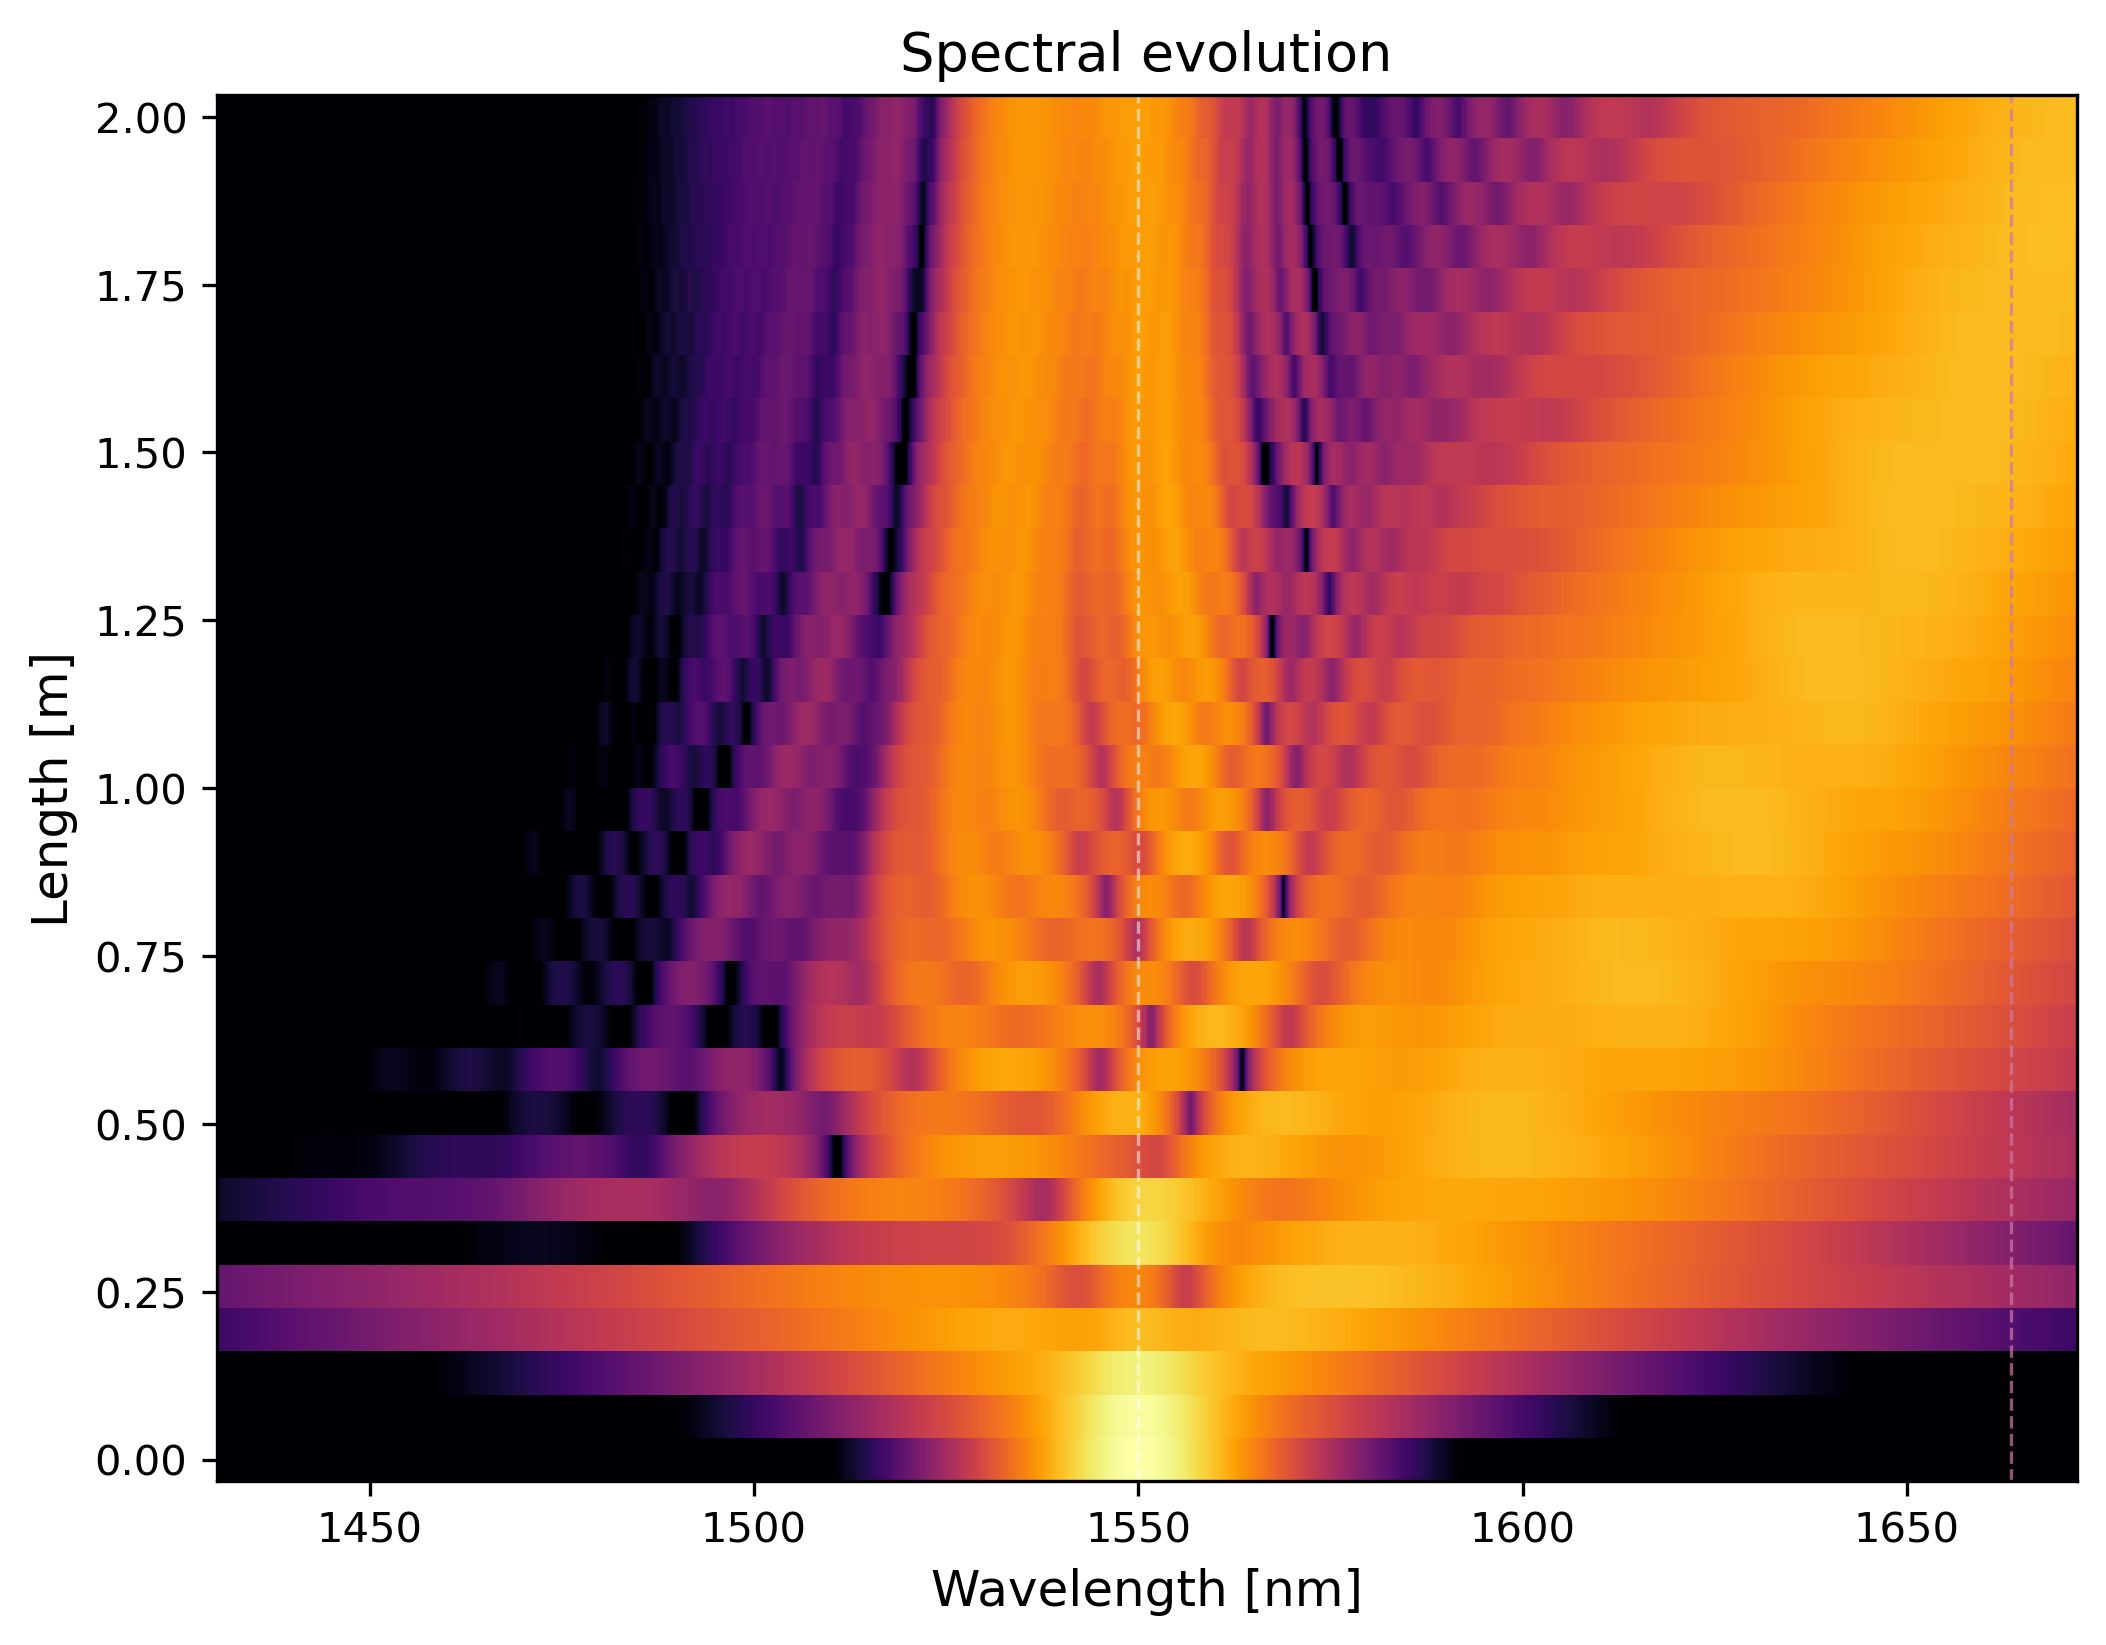
\includegraphics[height=0.31\textheight]{figures/control_smf28_no_shaping_evolution.png}
\caption{No-optimization control for the canonical SMF-28 setting. The flat
phase is the reference group: it shows the spectral evolution before recovery
or saddle diagnostics try to improve anything.}
\end{figure}

\begin{figure}[p]
\centering
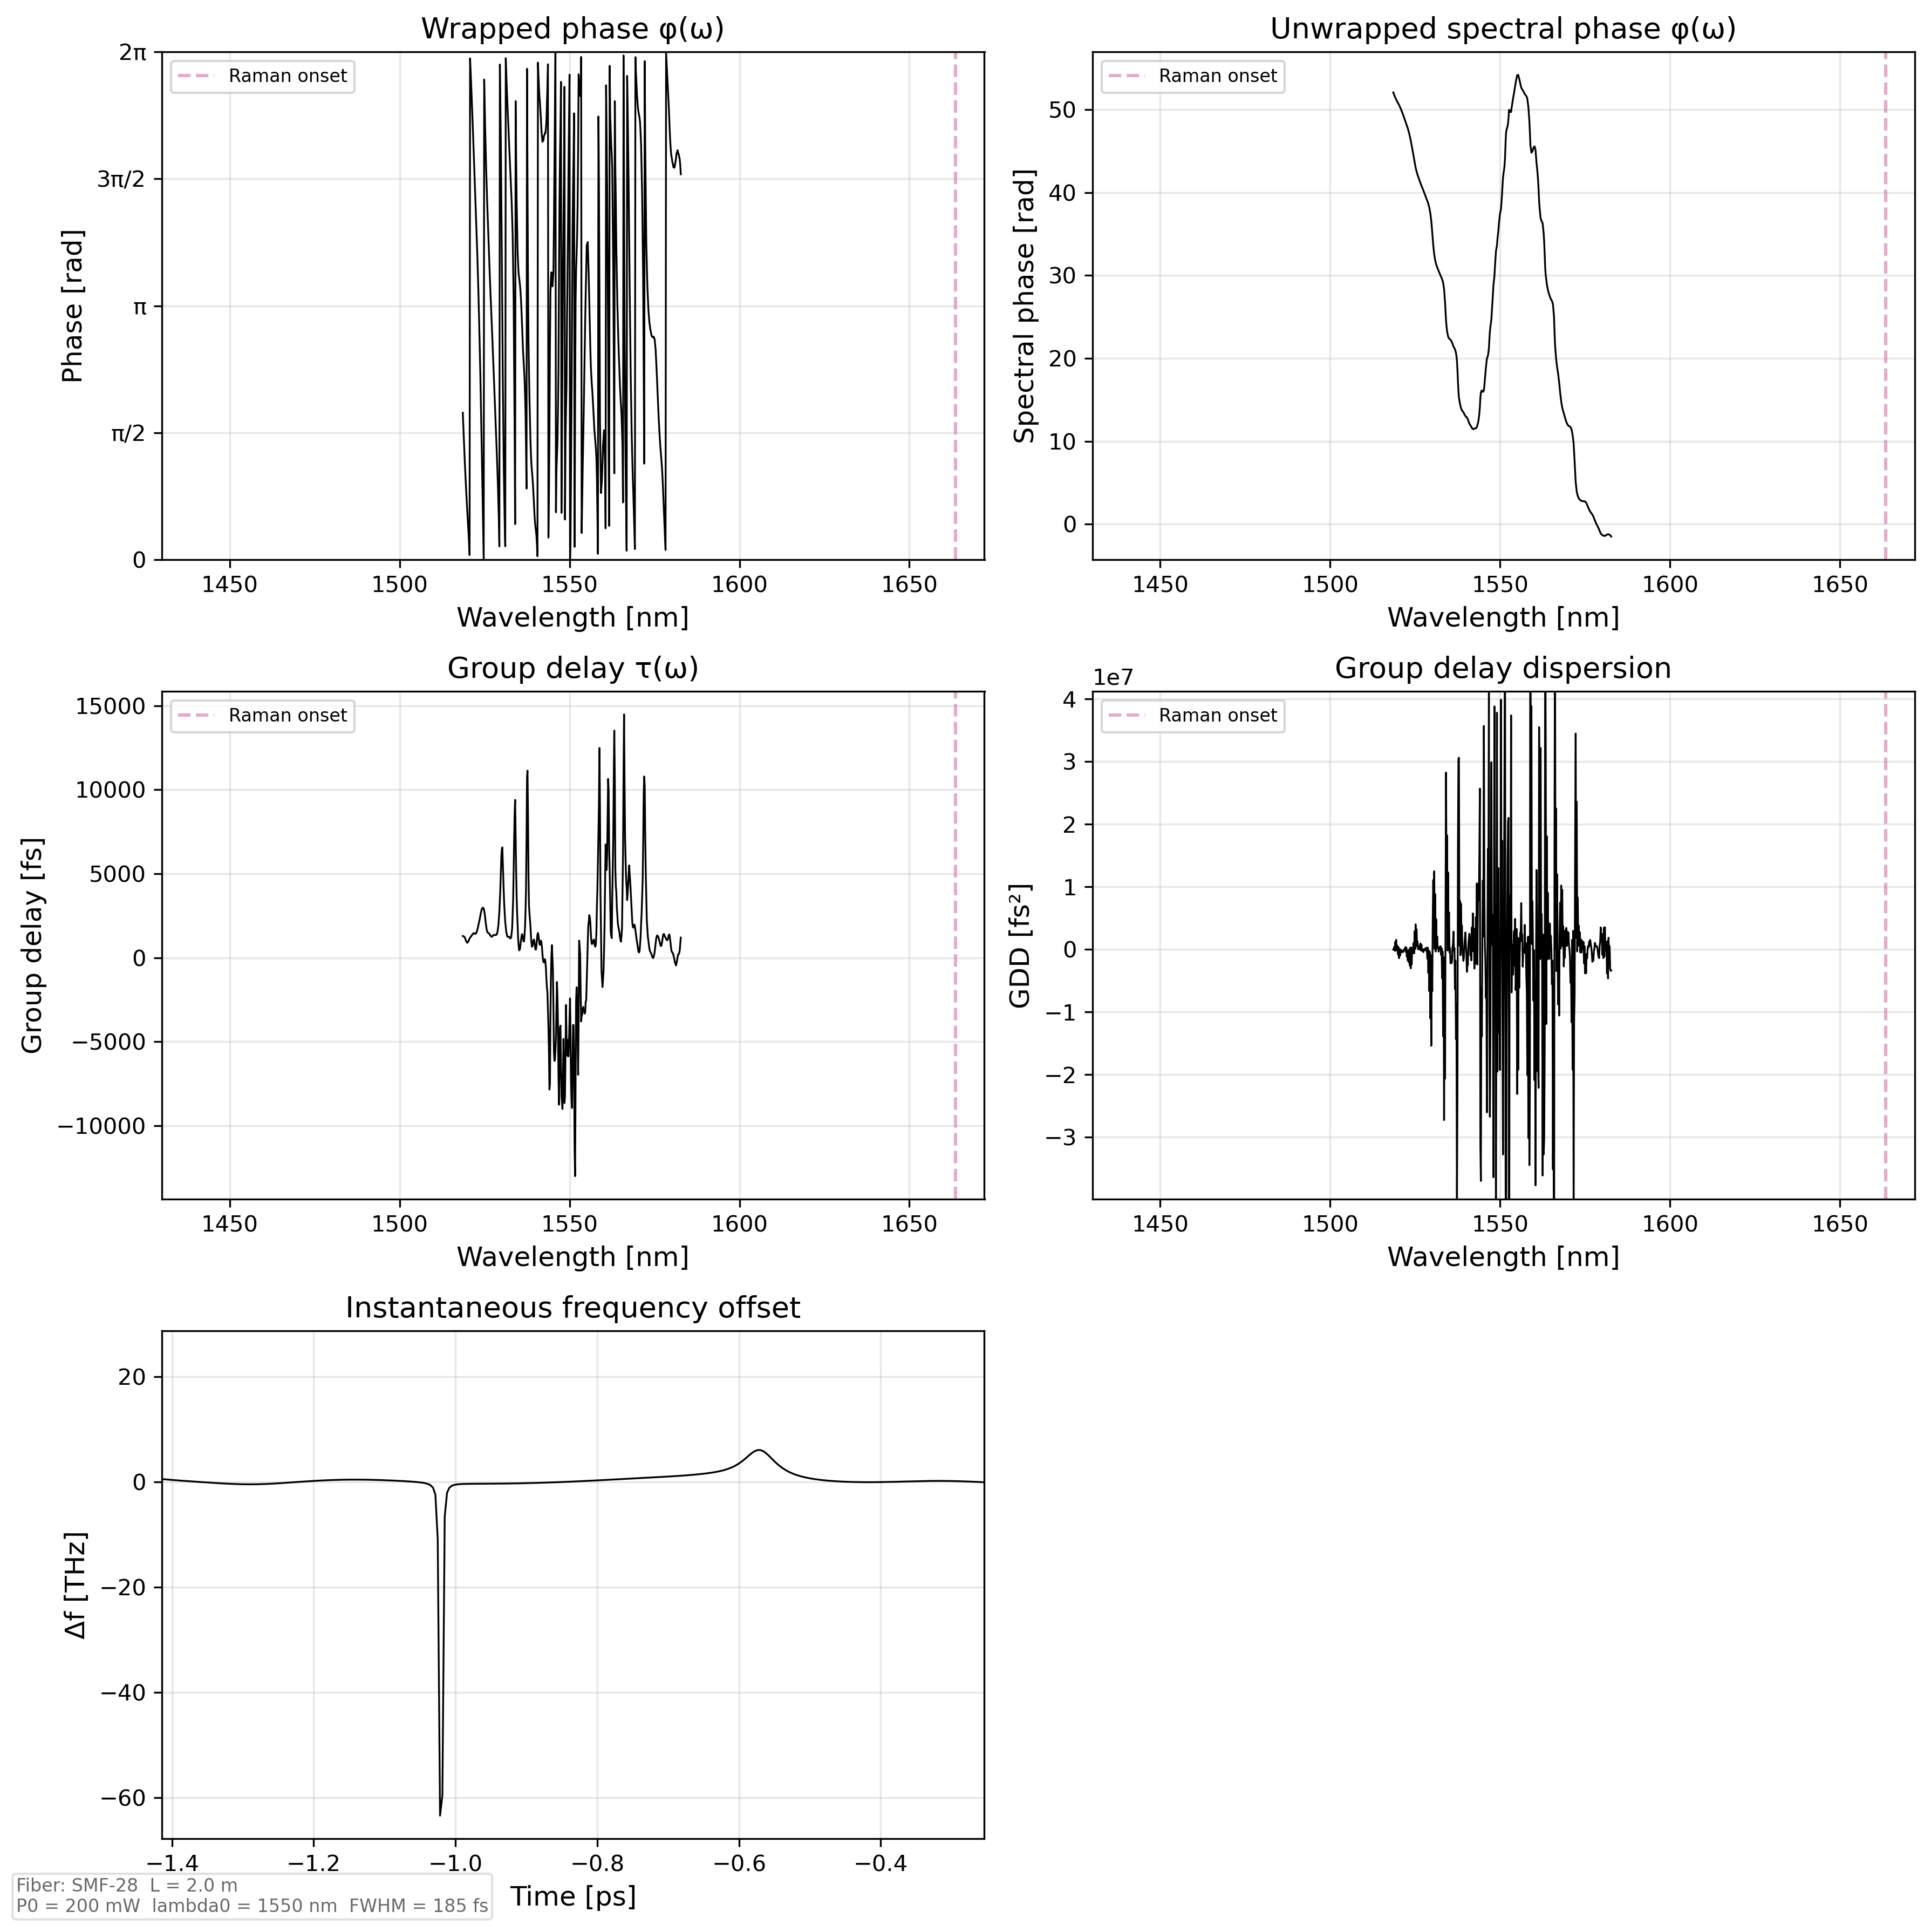
\includegraphics[height=0.47\textheight]{figures/recovered_smf28_phase_diagnostic.png}
\vspace{0.5em}

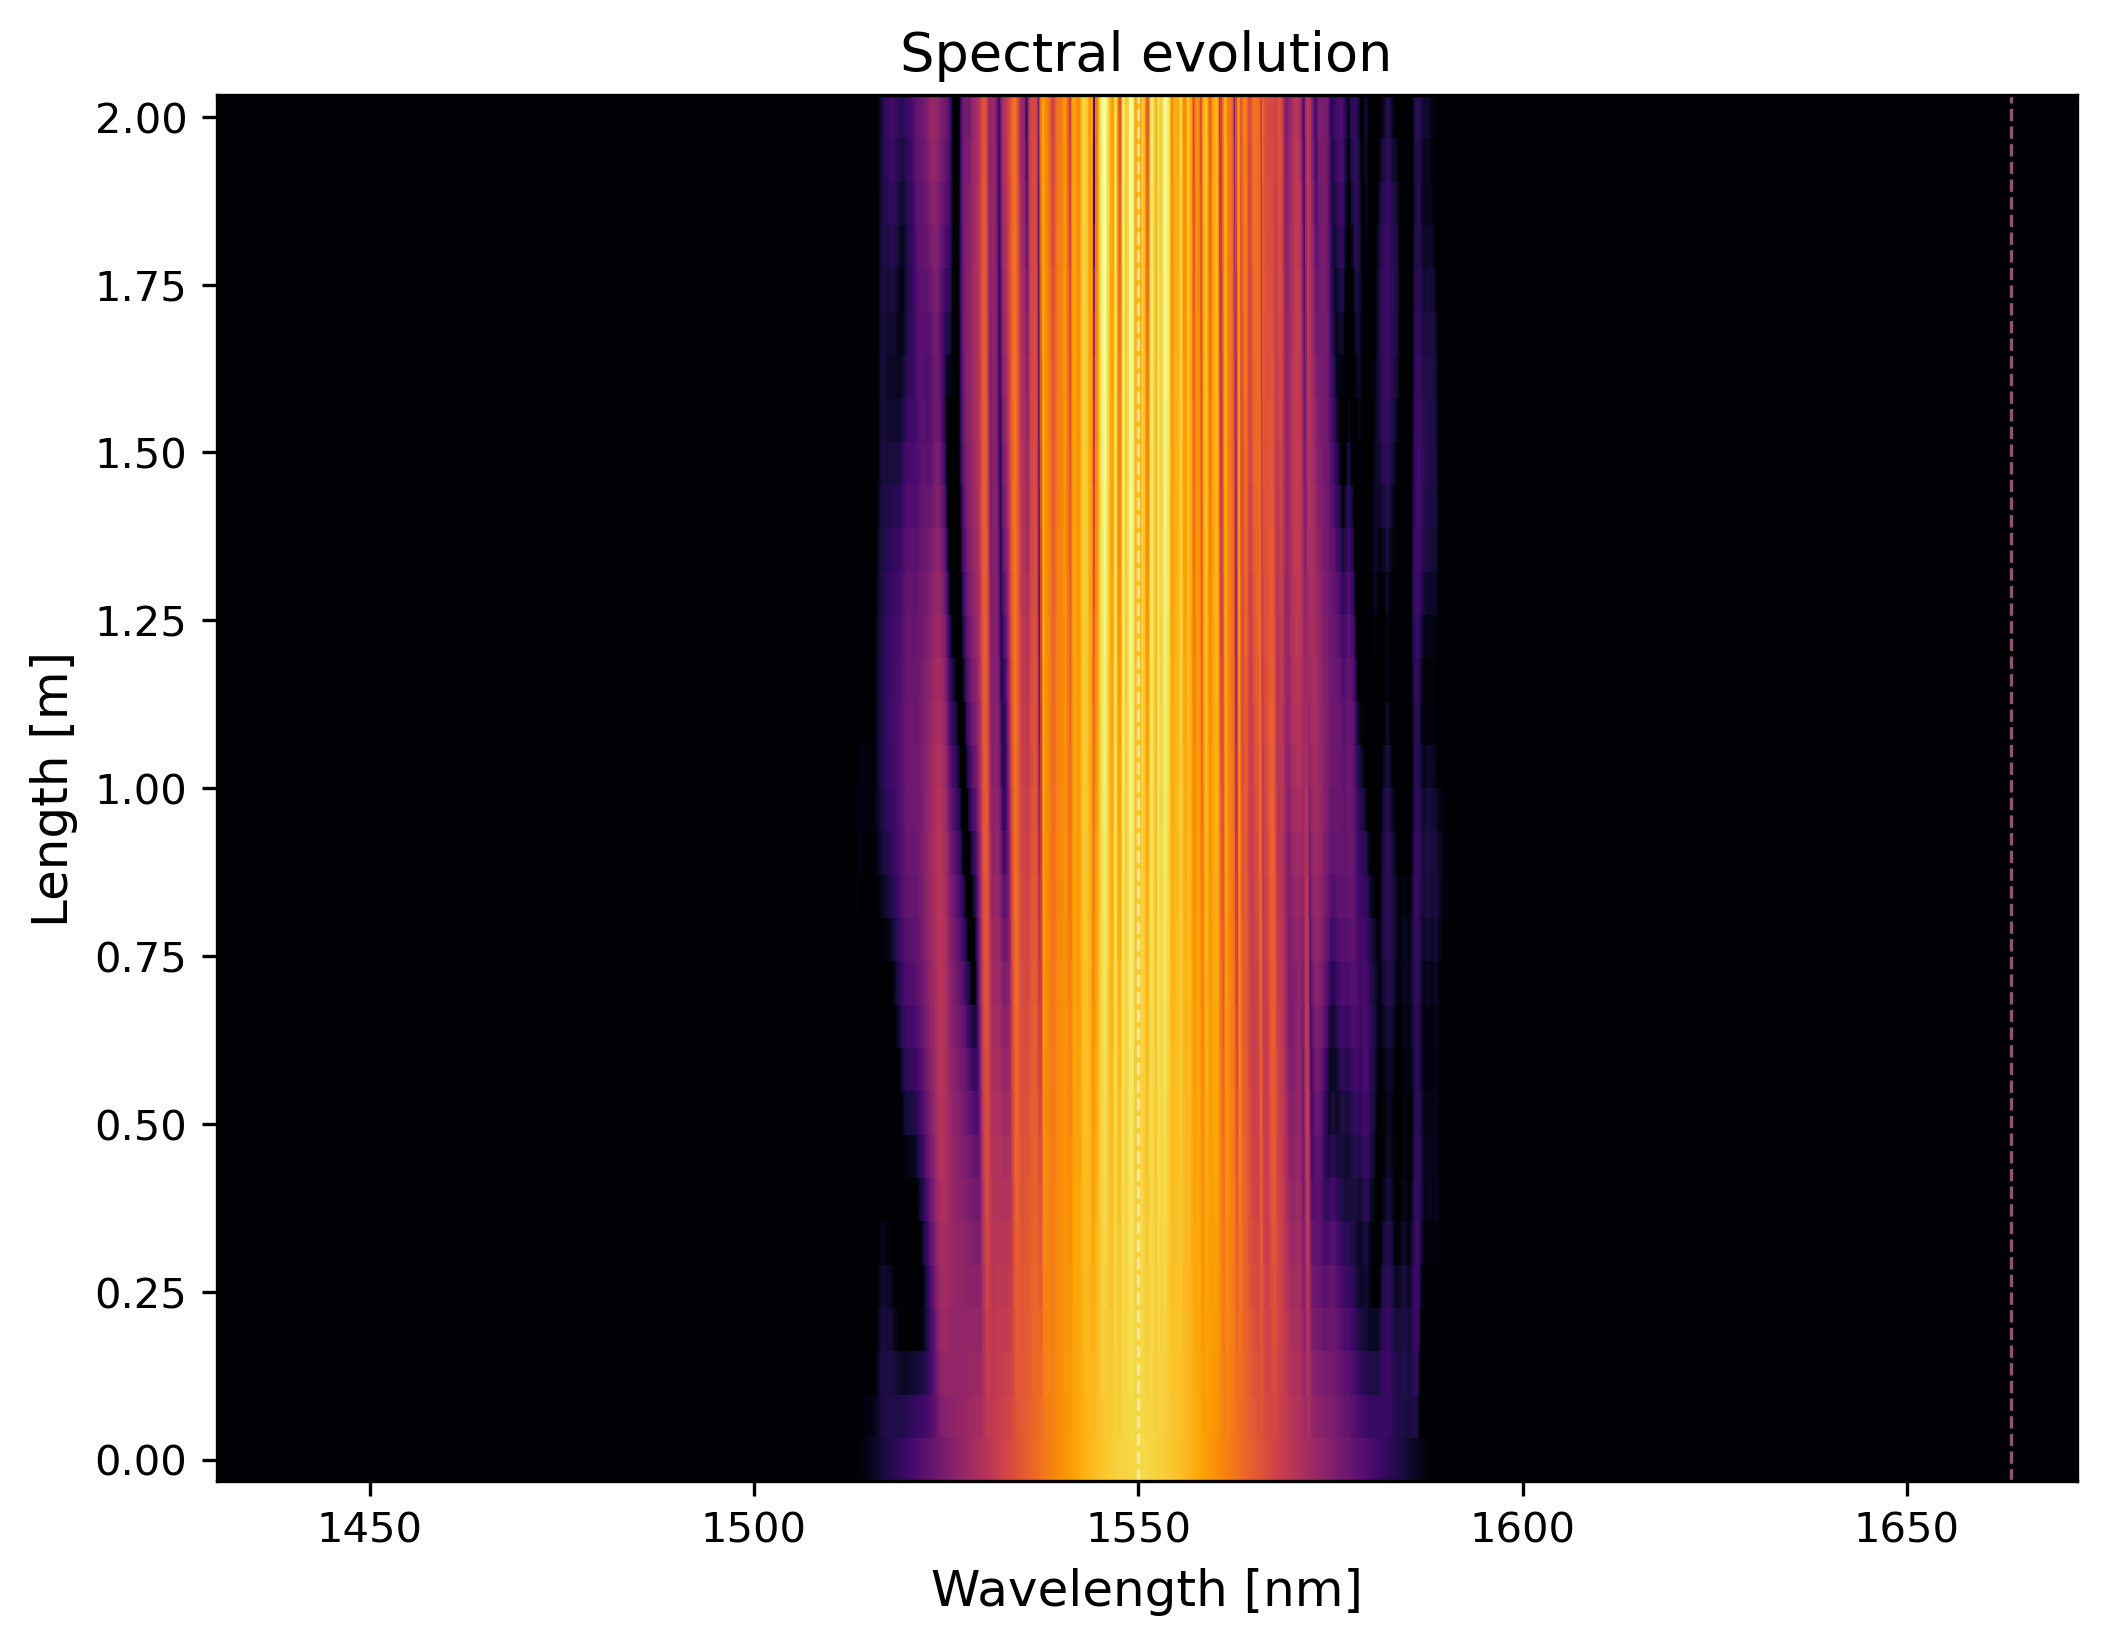
\includegraphics[height=0.31\textheight]{figures/recovered_smf28_evolution.png}
\caption{Recovered SMF-28 anchor. This is the cleanest recovered single-mode
case in the note: it passes the boundary gate, converges, and keeps the
standard phase-diagnostic plus heat-map evidence together.}
\end{figure}

\begin{figure}[p]
\centering
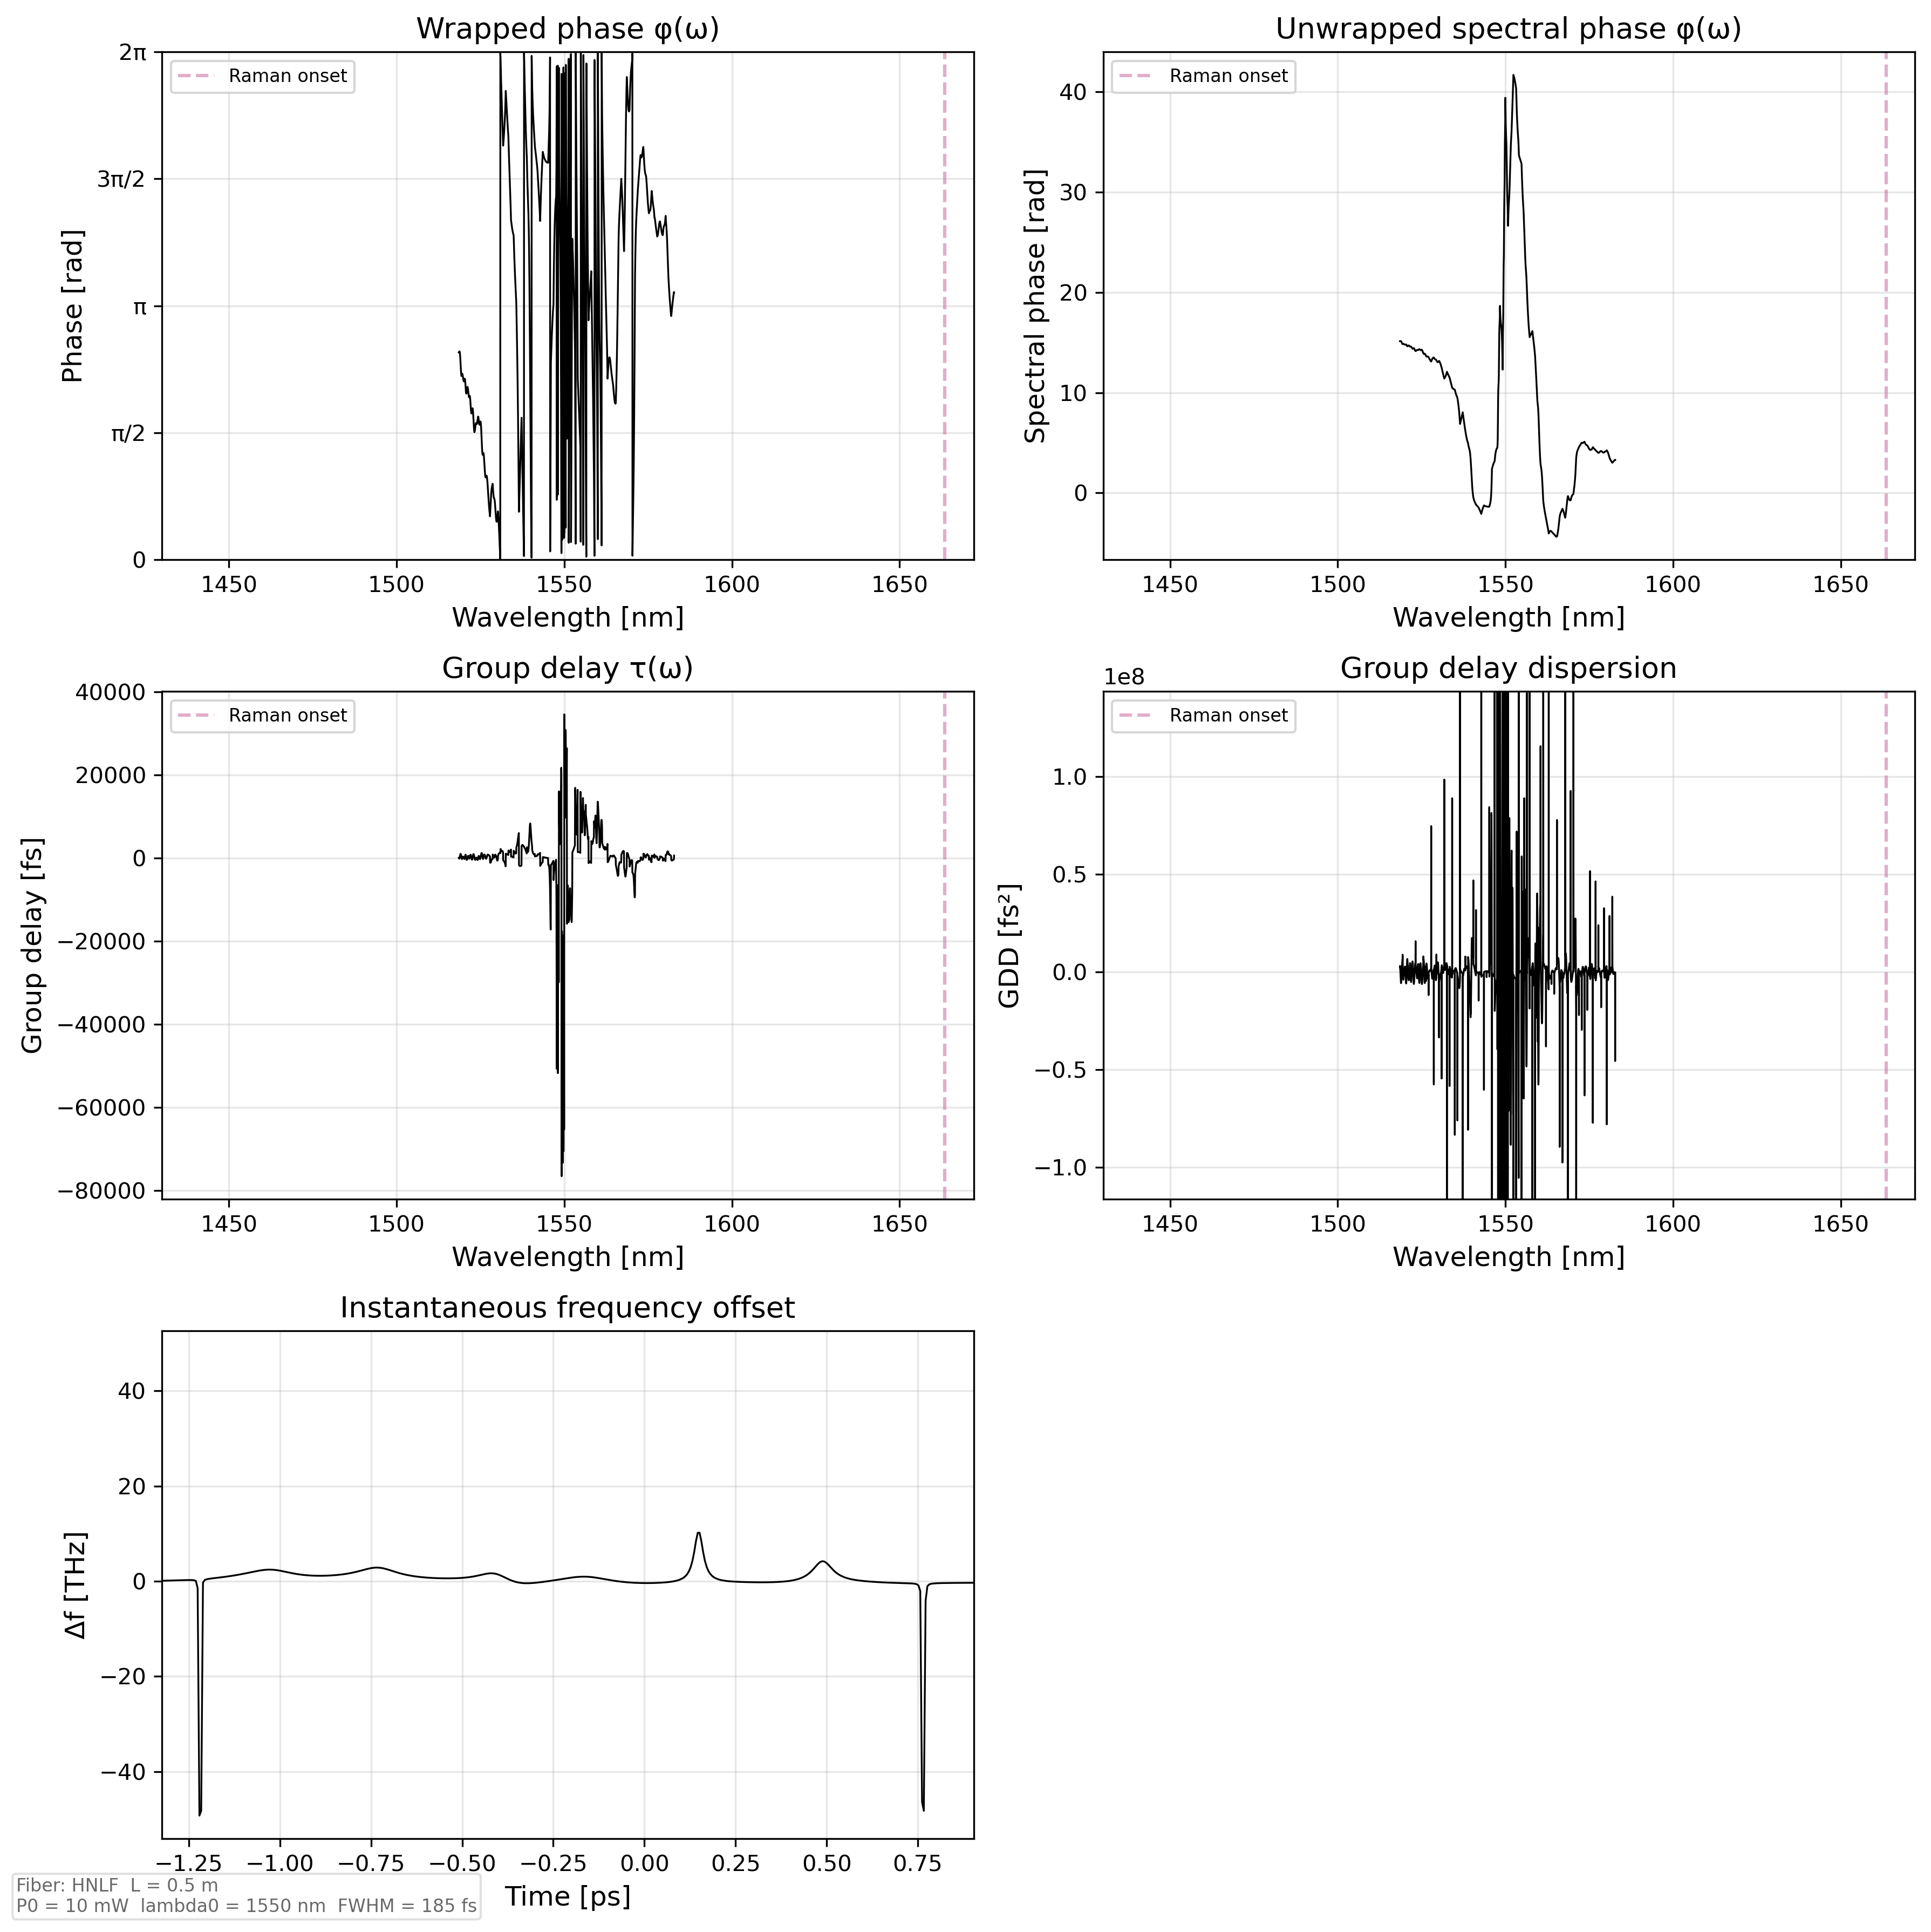
\includegraphics[height=0.47\textheight]{figures/recovered_hnlf_phase_diagnostic.png}
\vspace{0.5em}

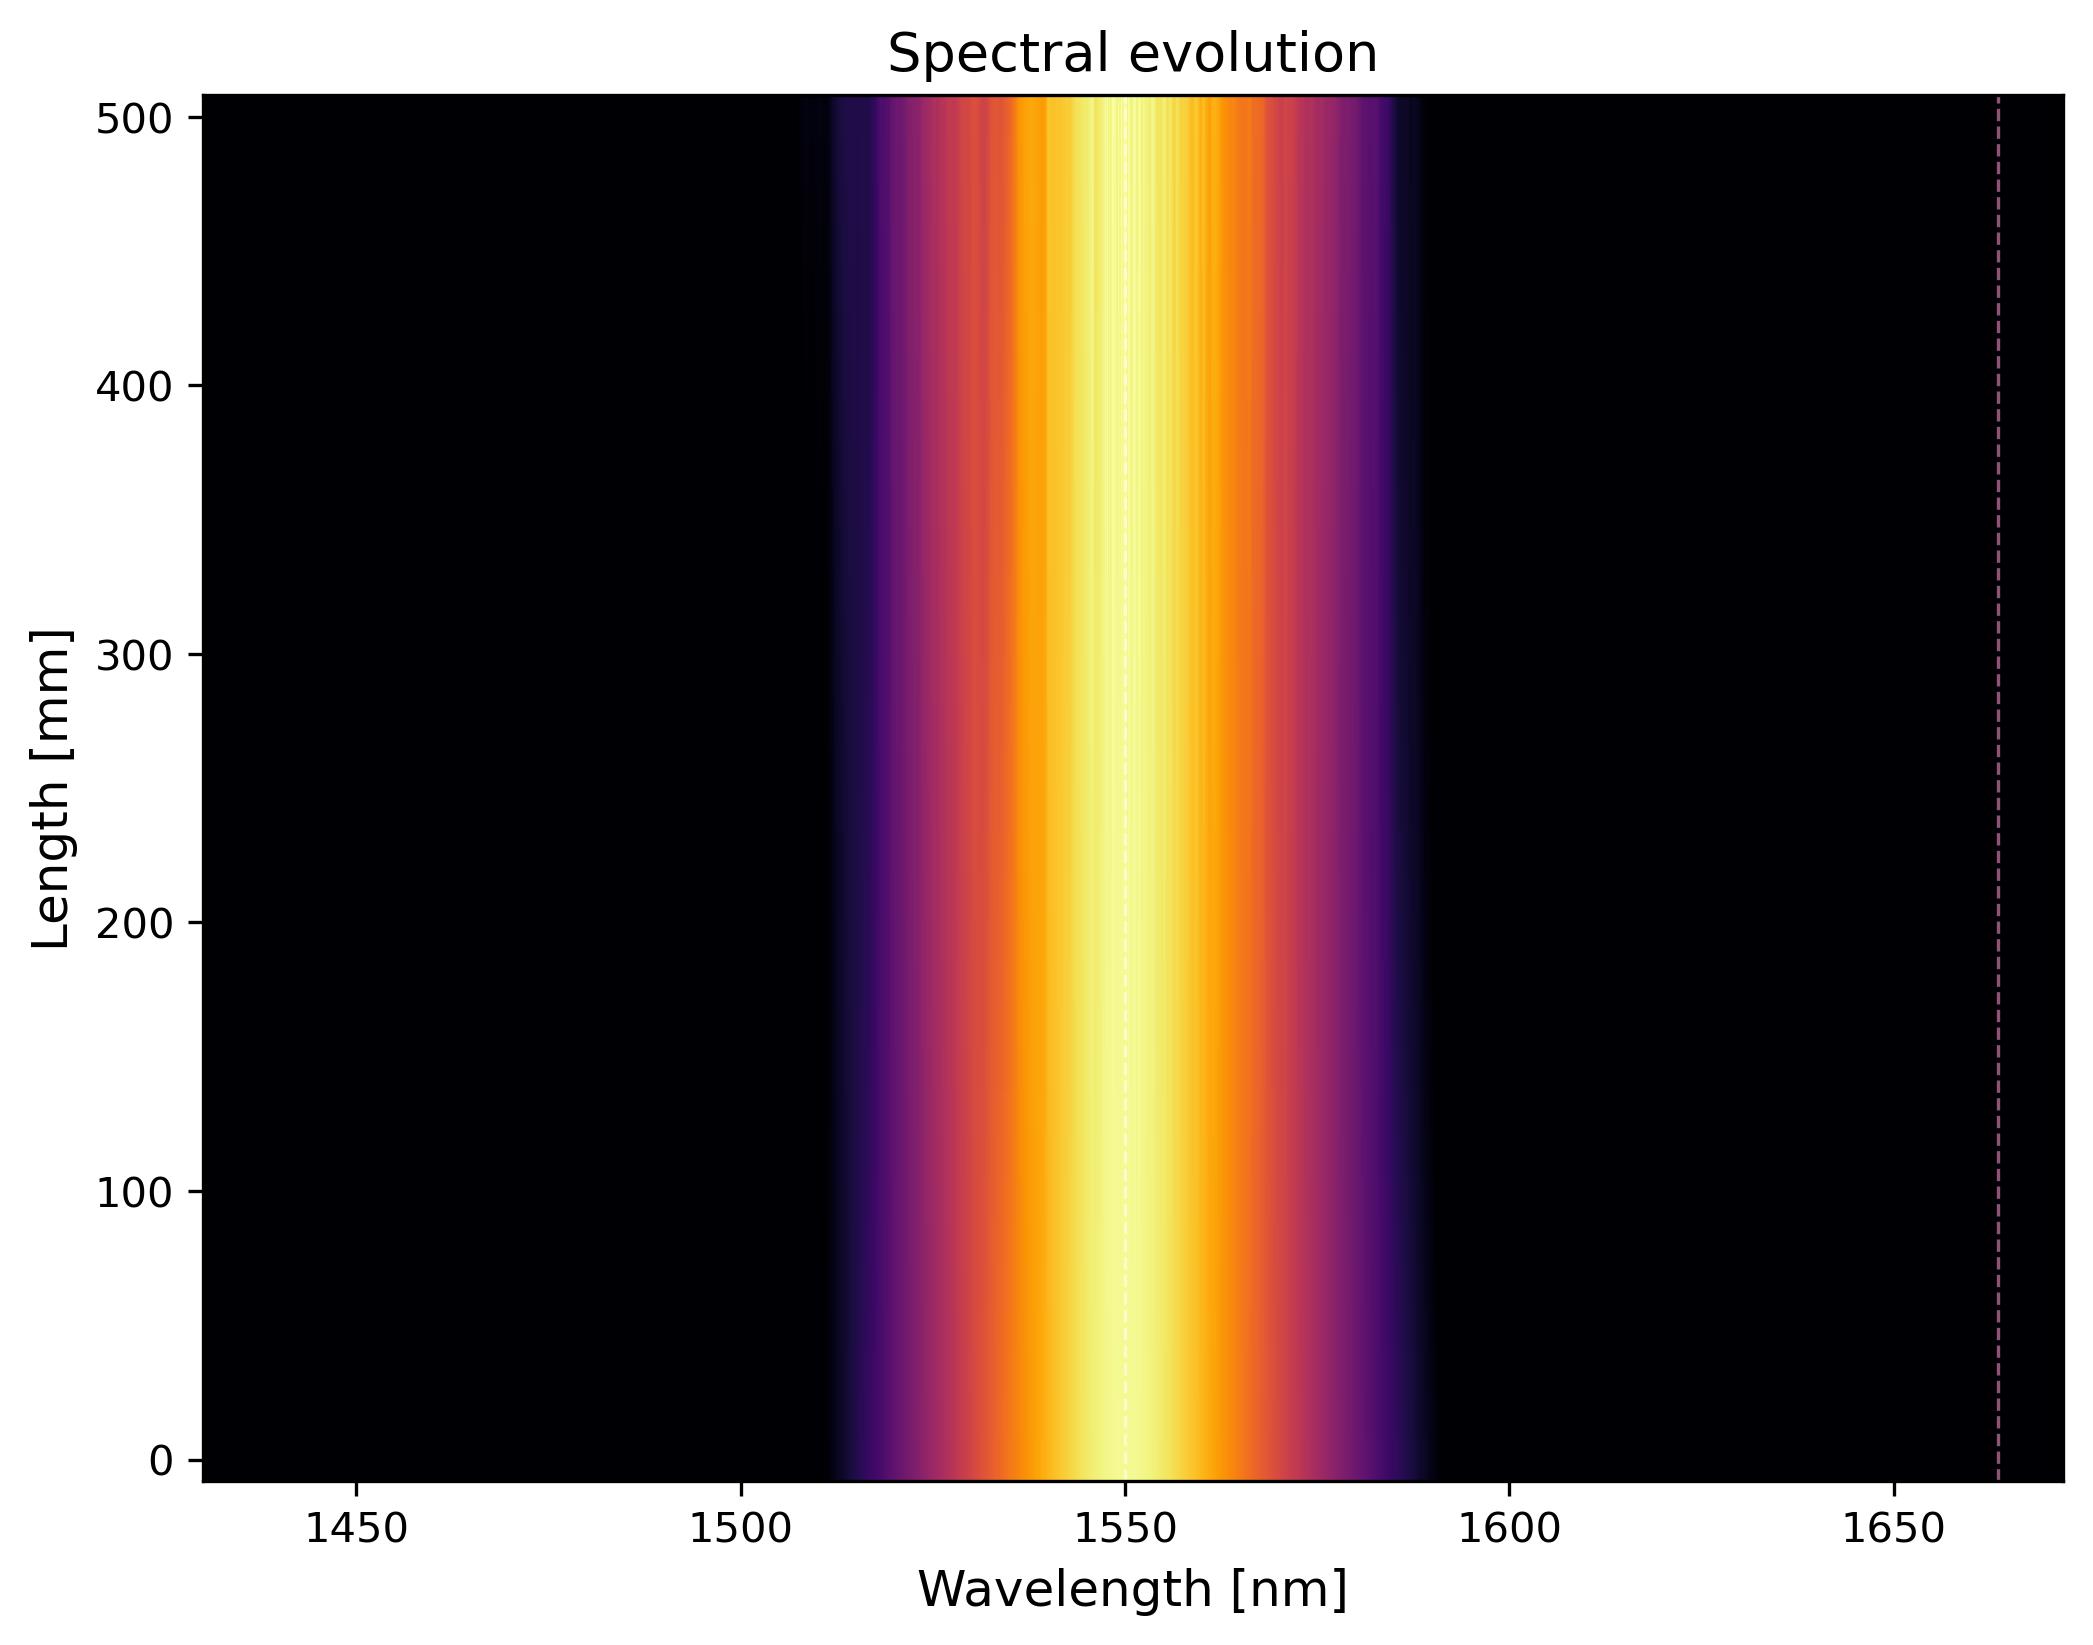
\includegraphics[height=0.31\textheight]{figures/recovered_hnlf_evolution.png}
\caption{Recovered HNLF anchor. The value is very deep and the edge fraction is
inside the gate, but the optimizer hit its iteration cap, so this page supports
an achieved-value claim rather than an optimum claim.}
\end{figure}

\begin{figure}[p]
\centering
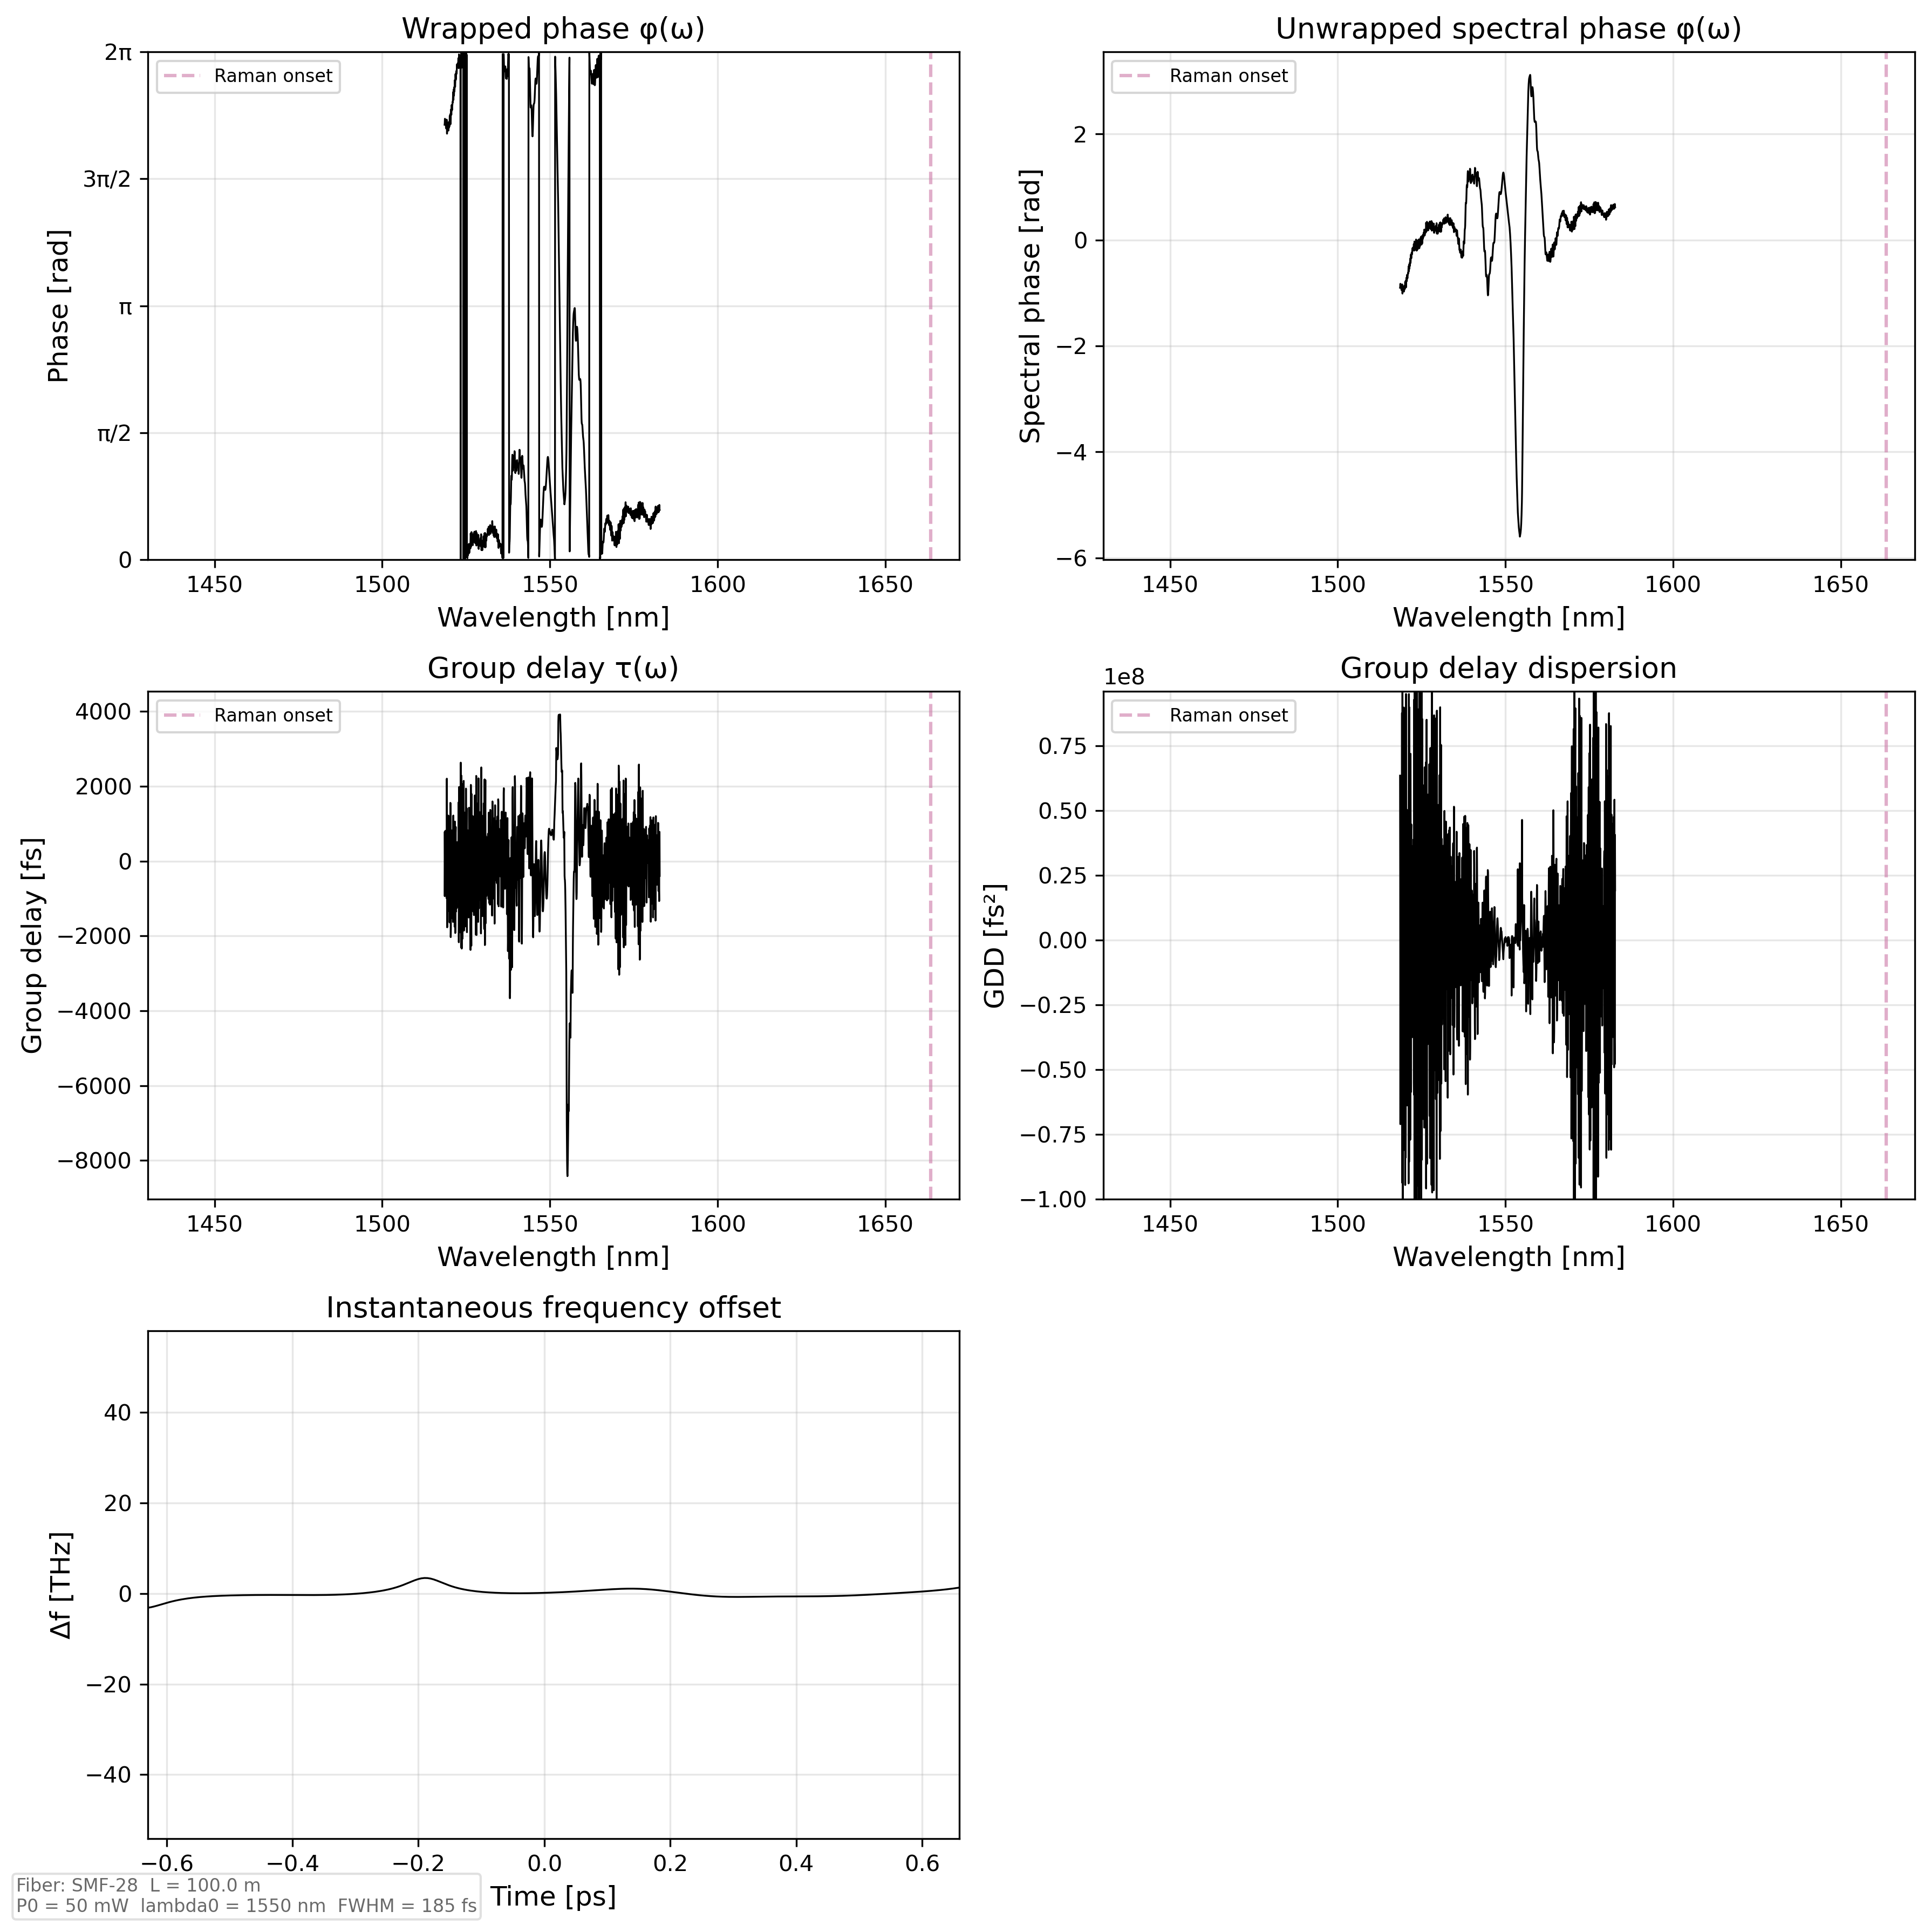
\includegraphics[height=0.47\textheight]{figures/validated_longfiber_phase_diagnostic.png}
\vspace{0.5em}

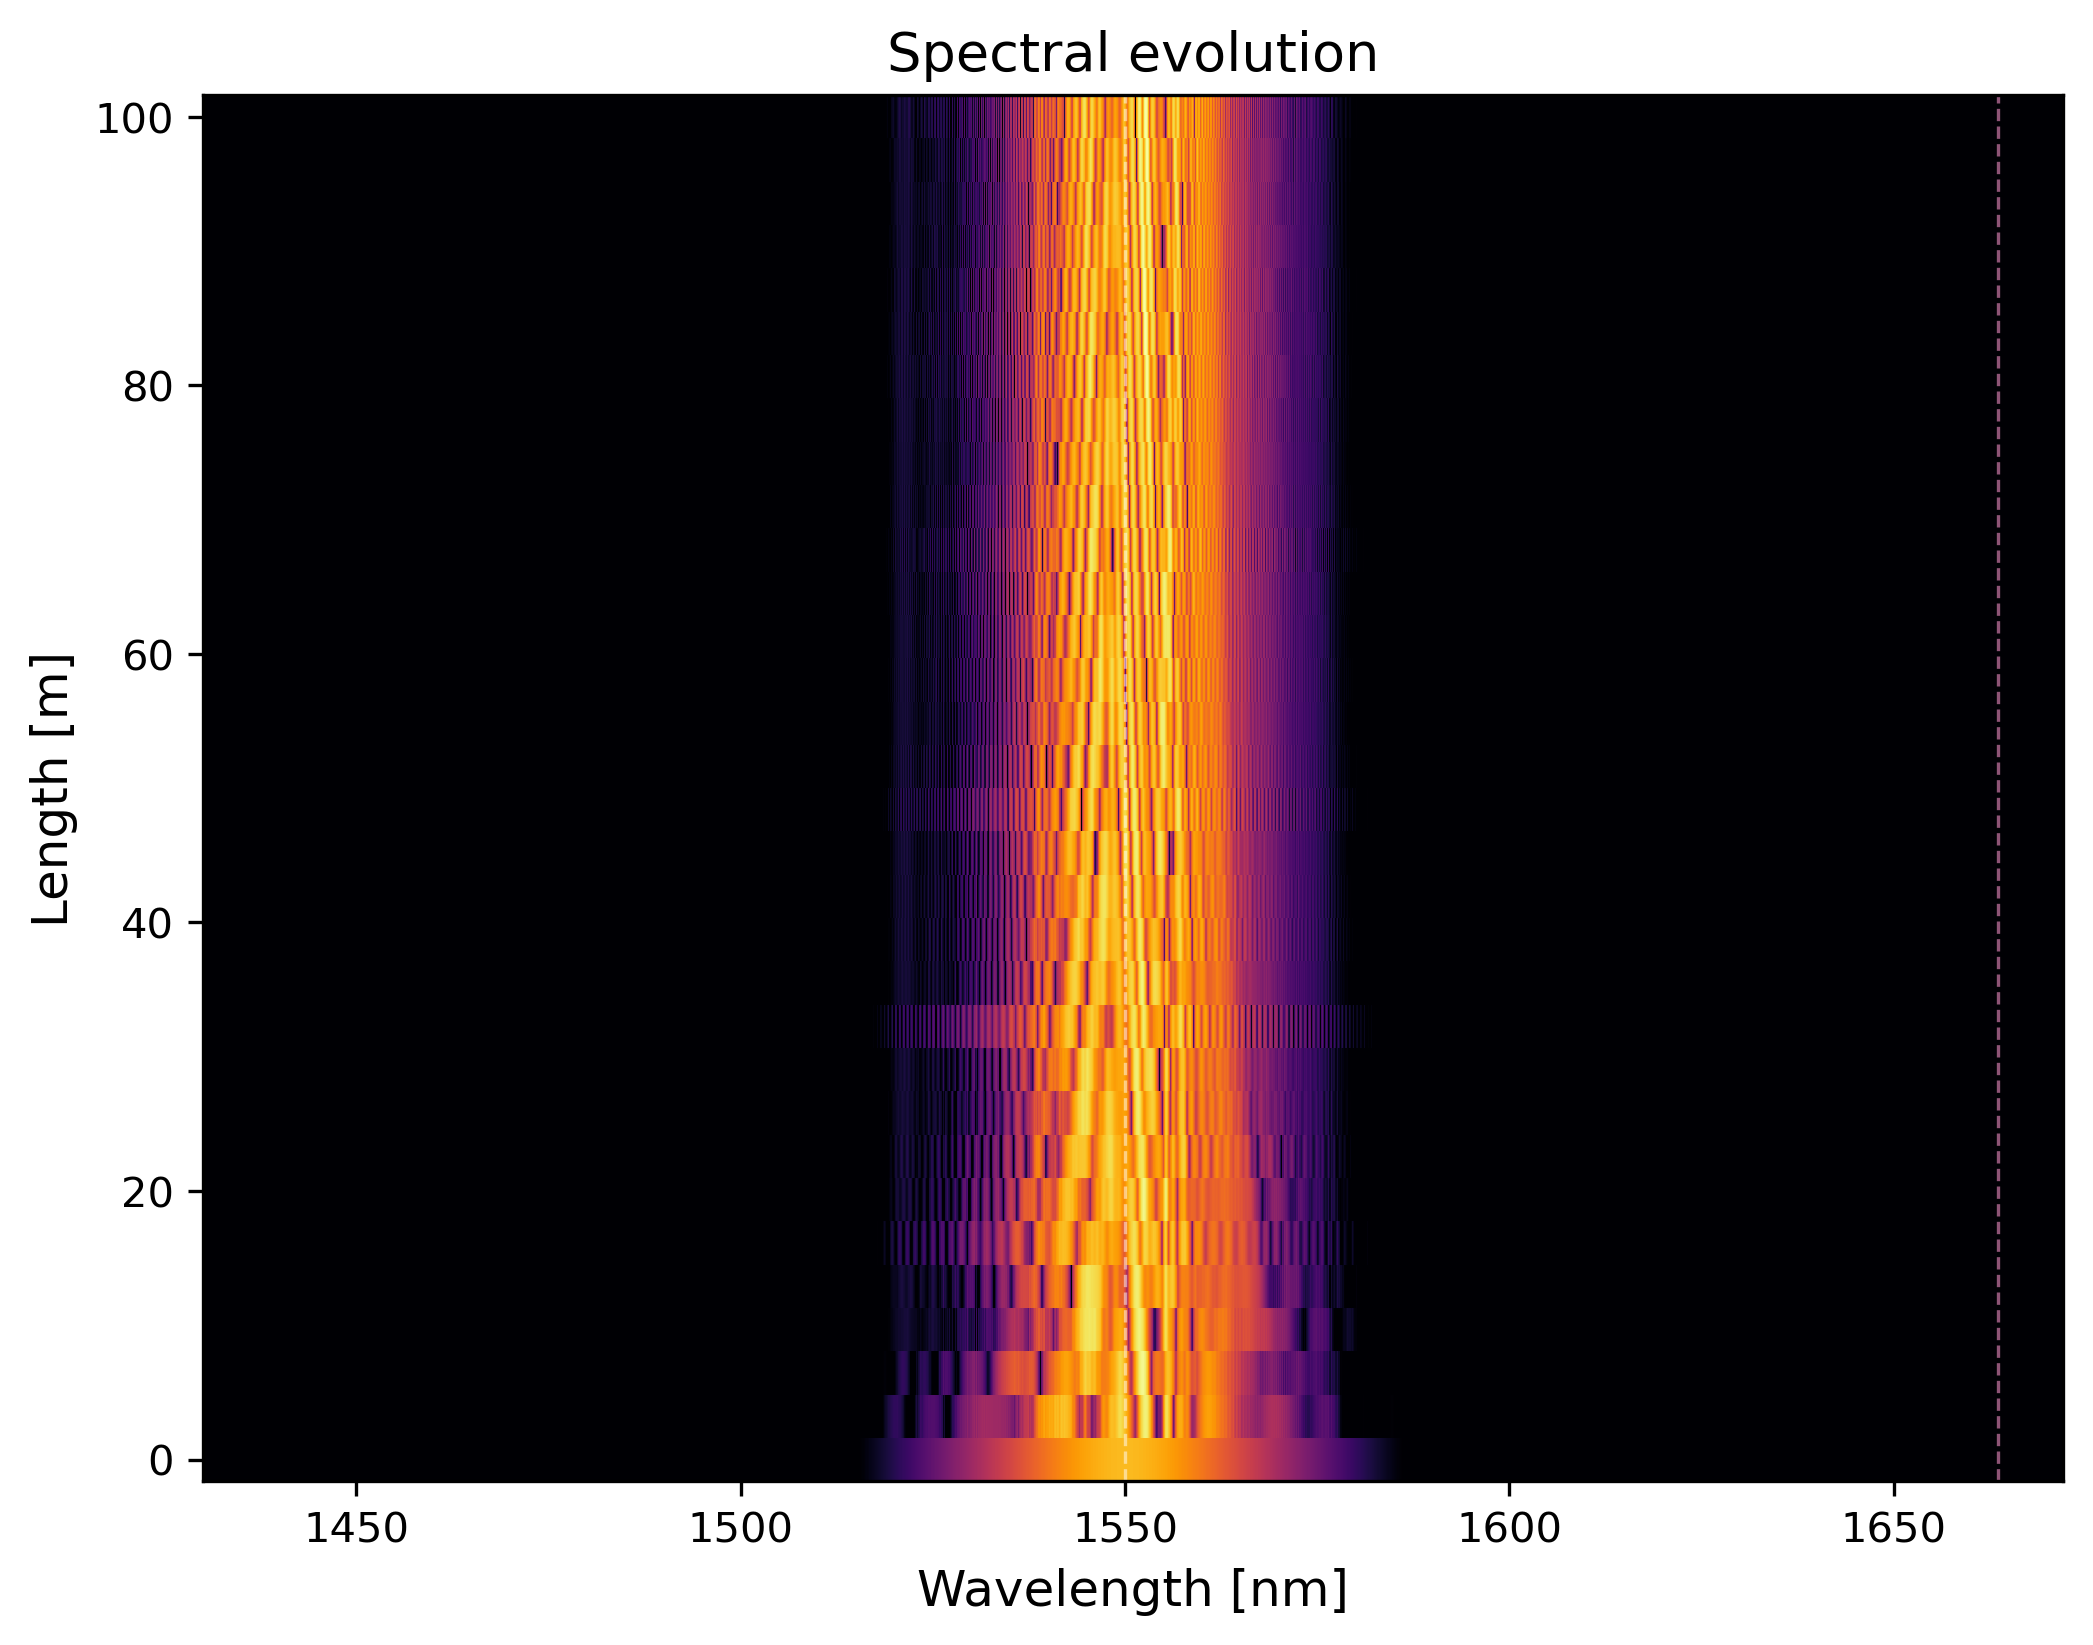
\includegraphics[height=0.31\textheight]{figures/validated_longfiber_evolution.png}
\caption{Validated long-fiber lower bound. The long propagation is numerically
contained, but the stored run should be described as a validated achieved
value, not as a solved global or local optimum.}
\end{figure}

\begin{figure}[p]
\centering
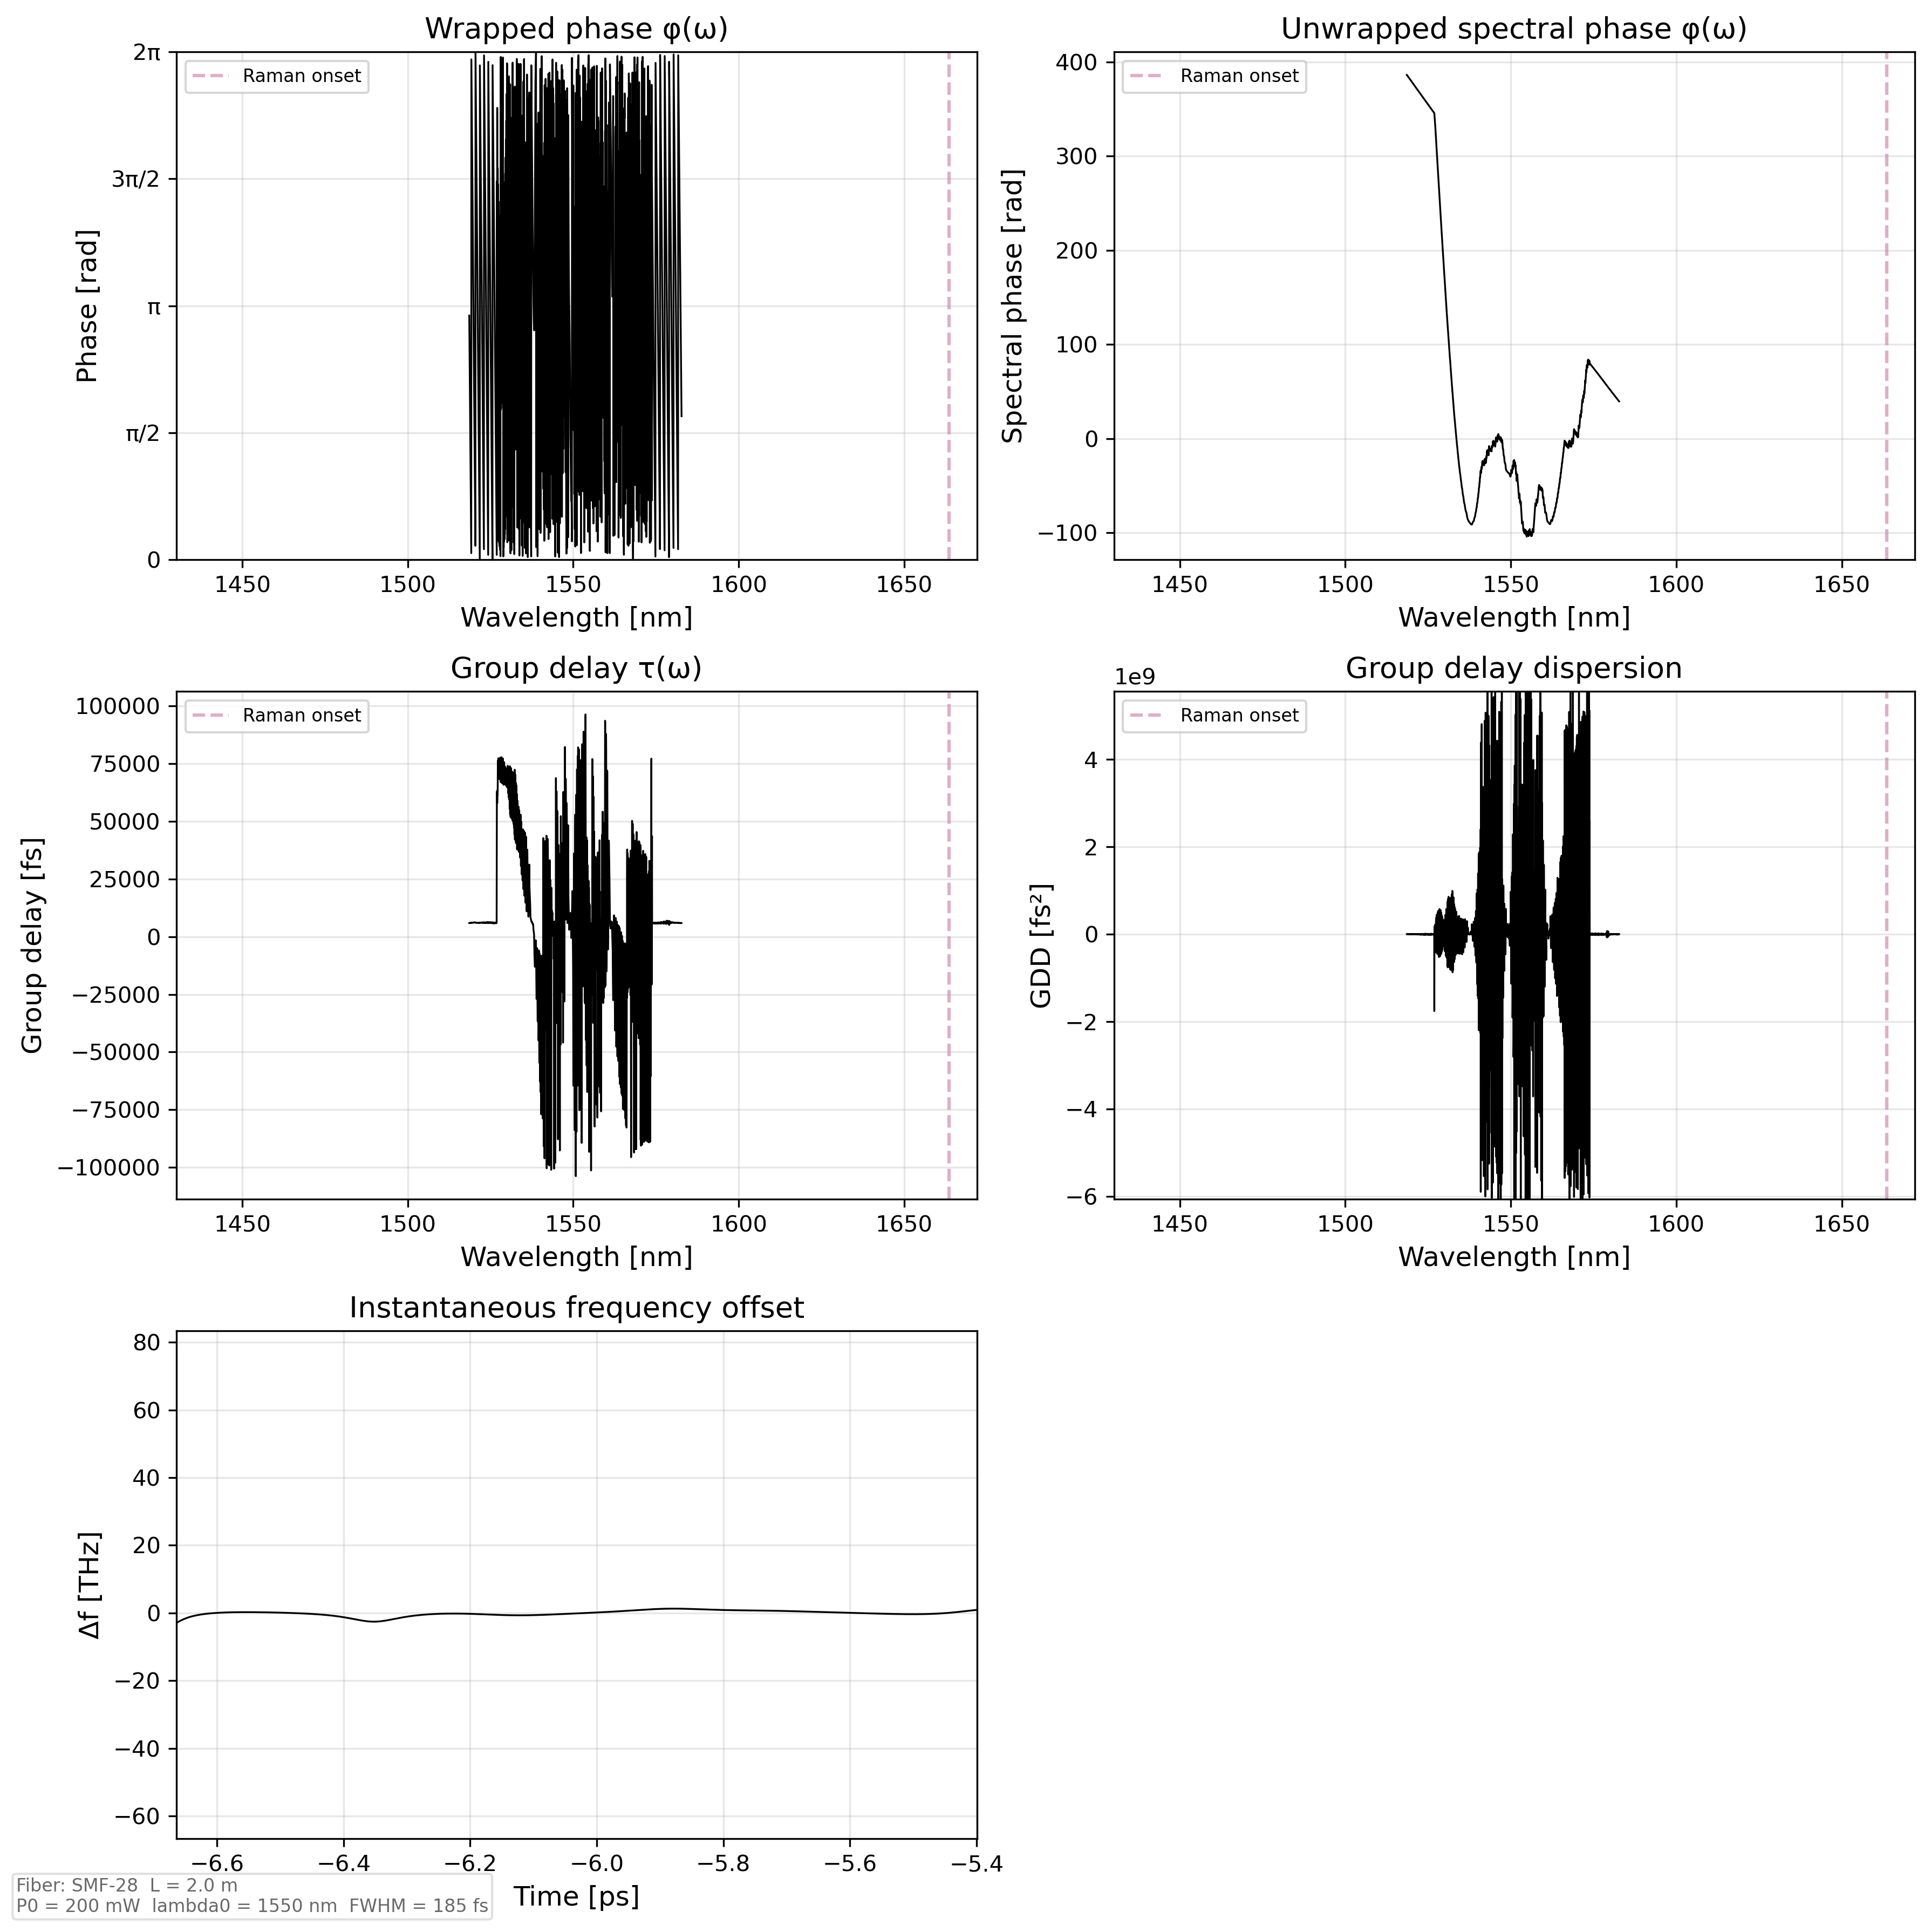
\includegraphics[height=0.47\textheight]{figures/retired_sweep_fullgrid_phase_diagnostic.png}
\vspace{0.5em}

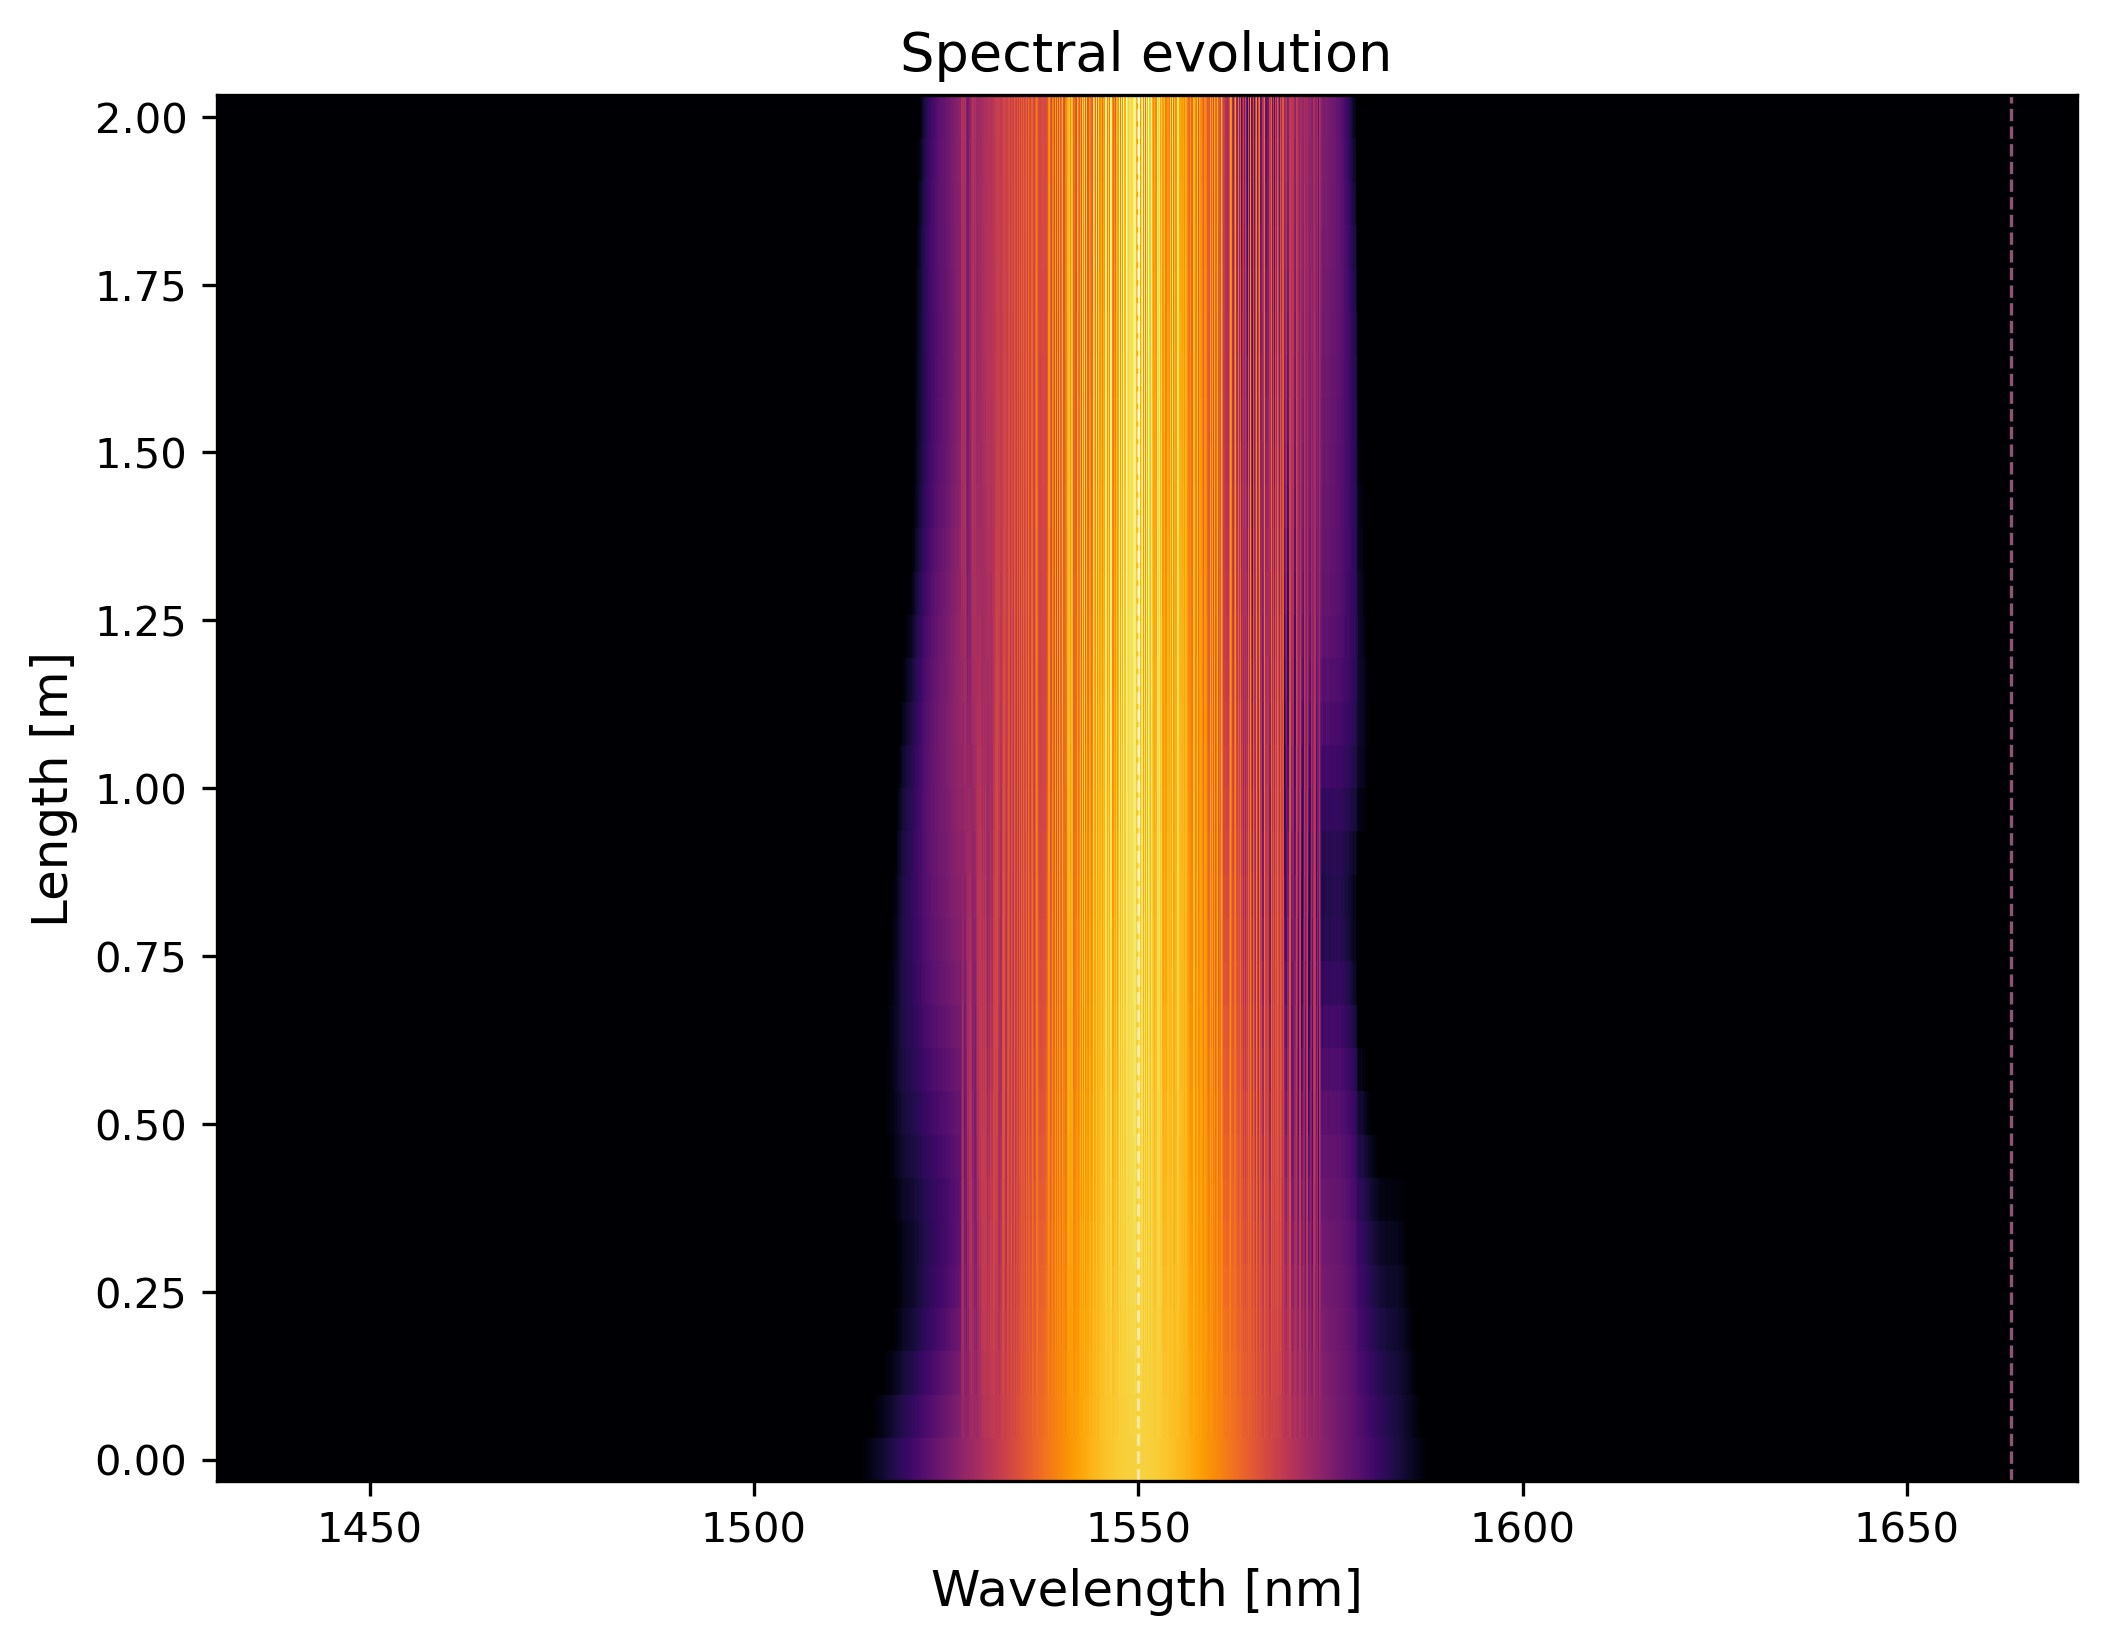
\includegraphics[height=0.31\textheight]{figures/retired_sweep_fullgrid_evolution.png}
\caption{Best recovered point from the retired simple-control sweep. The
objective is deep, but the edge fraction is far above the acceptance gate, so
this image belongs in the note as a warning example rather than as a headline
success.}
\end{figure}

\clearpage
\section{The Retired Sweep}

The simple-control sweep was originally attractive because it suggested a clean
story: only a modest number of phase controls might be needed to reach nearly
full-grid suppression. Recovery made that story weaker. Even on a much larger
time window, the recovered sweep points kept too much energy near the boundary.

\begin{figure}[H]
\centering
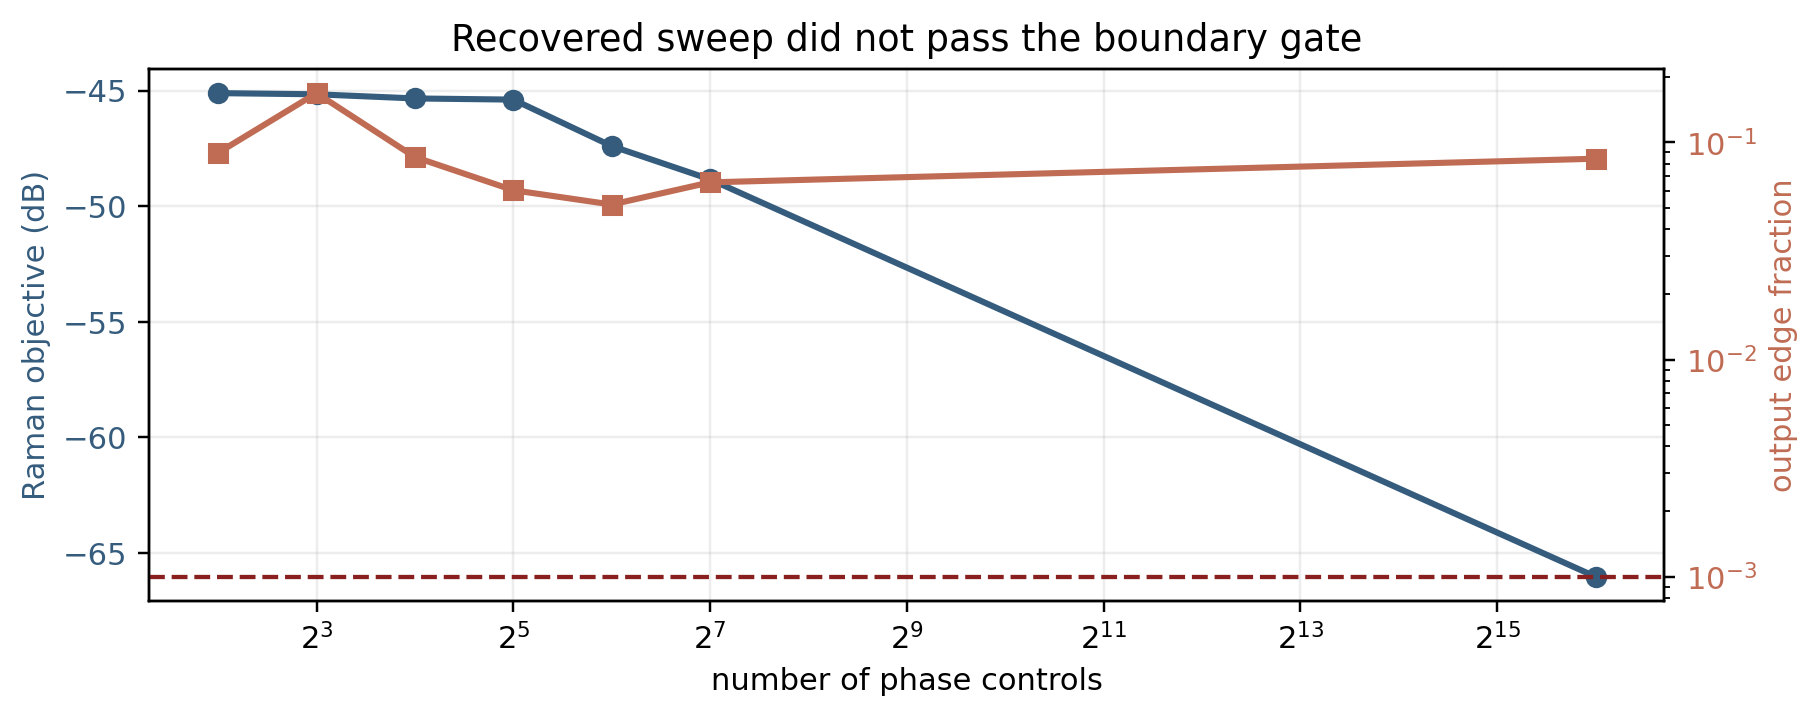
\includegraphics[width=0.92\linewidth]{figures/retired_sweep_recovery_summary.png}
\caption{Recovered simple-control sweep. The best objective comes from the
largest control space, but all recovered points remain well above the
\(10^{-3}\) edge-fraction gate. The right scientific move is to retire the
clean simplicity claim until a boundary-aware rerun proves it.}
\end{figure}

\subsection*{Intuition Check}

This is not a failed project result. It is a successful audit result. It tells
us not to build a public claim on a run that may have learned the simulation
window.

\section{Saddle Diagnostics}

Recovery tells us whether a point is numerically honest. It does not tell us
what kind of local geometry the optimizer found. For that, the project studies
the Hessian,
\[
    H(\phi)=\nabla^2_\phi \Jsurf(\phi).
\]
For a perturbation \(v\), the local quadratic model is
\[
    \Jsurf(\phi+\epsilon v)
    \approx
    \Jsurf(\phi)
    + \epsilon \nabla\Jsurf(\phi)^{T}v
    + \frac{\epsilon^2}{2}v^T H(\phi)v.
\]
At a stationary point, the gradient term is small. The sign of \(v^THv\) then
decides whether that direction bends upward or downward.

\begin{itemize}
    \item If all non-gauge eigenvalues are positive, the point is minimum-like.
    \item If some are positive and some are negative, the point is saddle-like.
    \item If the negative eigenvalues are small, first-order optimizers may
    stop there even though a downhill direction exists.
\end{itemize}

\begin{figure}[H]
\centering
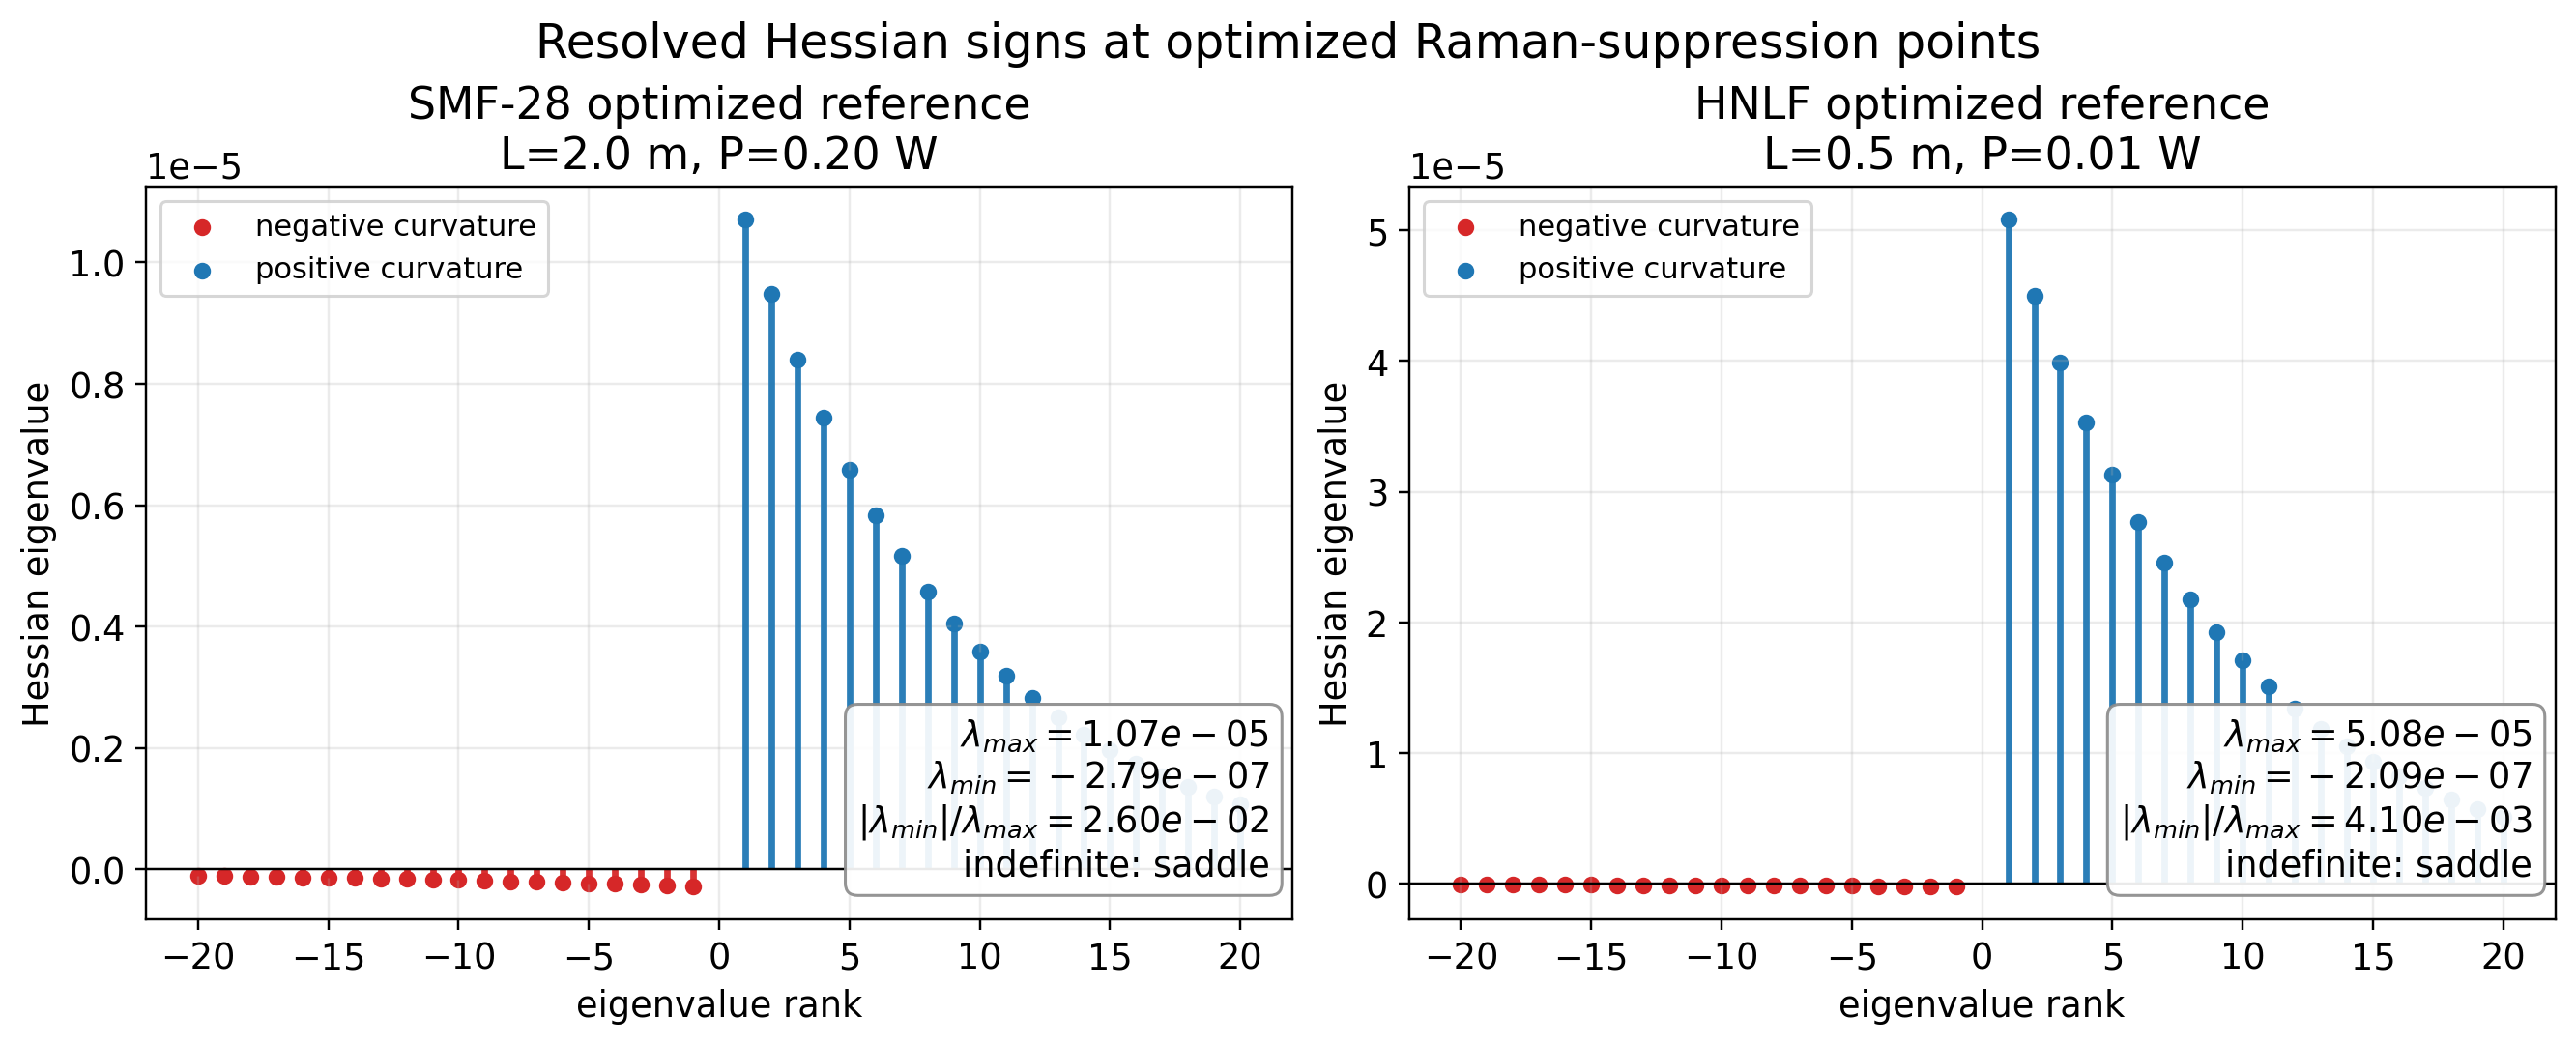
\includegraphics[width=0.82\linewidth]{figures/hessian_saddle_spectrum_clean.png}
\caption{Resolved Hessian signs at optimized Raman-suppression points. The
presence of both positive and negative curvature is the signature of a saddle,
not a strict local minimum.}
\end{figure}

\subsection*{Intuition Check}

The Hessian is the local ``bowl test.'' A minimum is a bowl from every
direction. A saddle is a mountain pass: if you move one way it goes up, but if
you move another way it goes down.

\section{Control-Space Ladder}

The most useful saddle experiment restricts the phase to a small basis, then
opens the basis gradually. Let \(B\in\mathbb{R}^{\Nt\times \Nphi}\) be a basis
matrix and \(c\in\mathbb{R}^{\Nphi}\) be the coefficient vector:
\[
    \phi = Bc.
\]
The reduced objective is
\[
    f(c)=\Jsurf(Bc),
\]
with gradient and Hessian
\[
    \nabla_c f = B^T\nabla_\phi\Jsurf,
    \qquad
    \nabla_c^2 f \approx B^T H_\phi B
\]
plus the usual nonlinear terms from the dependence of the objective on
\(\phi\). In practice, the reduced Hessian can be computed densely for small
\(\Nphi\), which makes the local geometry much easier to classify.

\begin{figure}[H]
\centering
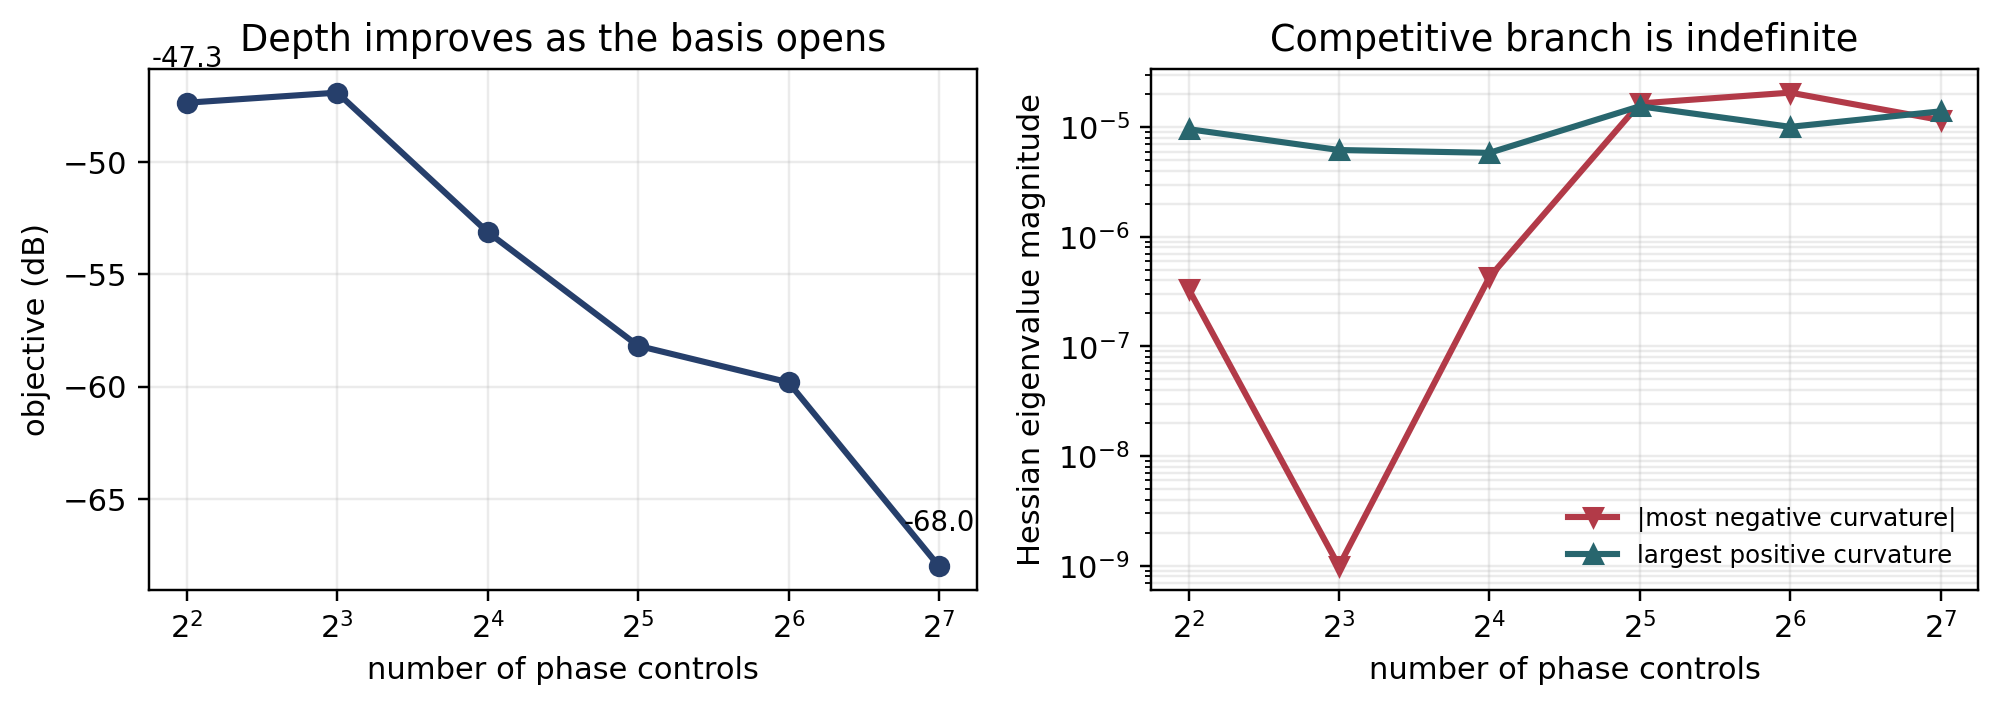
\includegraphics[width=0.94\linewidth]{figures/saddle_ladder_summary_clean.png}
\caption{Control-space ladder at the canonical SMF-28 setting. The very small
basis is minimum-like but shallow. The competitive branch appears once the
basis opens, and that branch is already indefinite.}
\end{figure}

The important result is not just that saddles exist. The important result is
where they appear. The minimum-like low-dimensional point is about
\(20\,\mathrm{dB}\) worse than the competitive branch. By the time the result
is competitive, the Hessian is already indefinite.

\subsection*{Intuition Check}

Restricting the basis is like forcing yourself to draw the phase mask with only
a few smooth knobs. That can create a clean local minimum, but it may be too
simple to get the best Raman suppression. Opening more knobs improves depth
and also opens directions where the landscape bends downward.

\section{Negative-Curvature Escape}

If the smallest Hessian eigenvalue is negative, then its eigenvector points
toward a local downhill direction in the quadratic model. A cheap escape
strategy is:
\[
    \phi_{\mathrm{new}}
    =
    \phi
    \pm \alpha v_{\min},
    \qquad
    H v_{\min}=\lambda_{\min}v_{\min},
    \qquad
    \lambda_{\min}<0,
\]
then restart the first-order optimizer.

\begin{figure}[H]
\centering
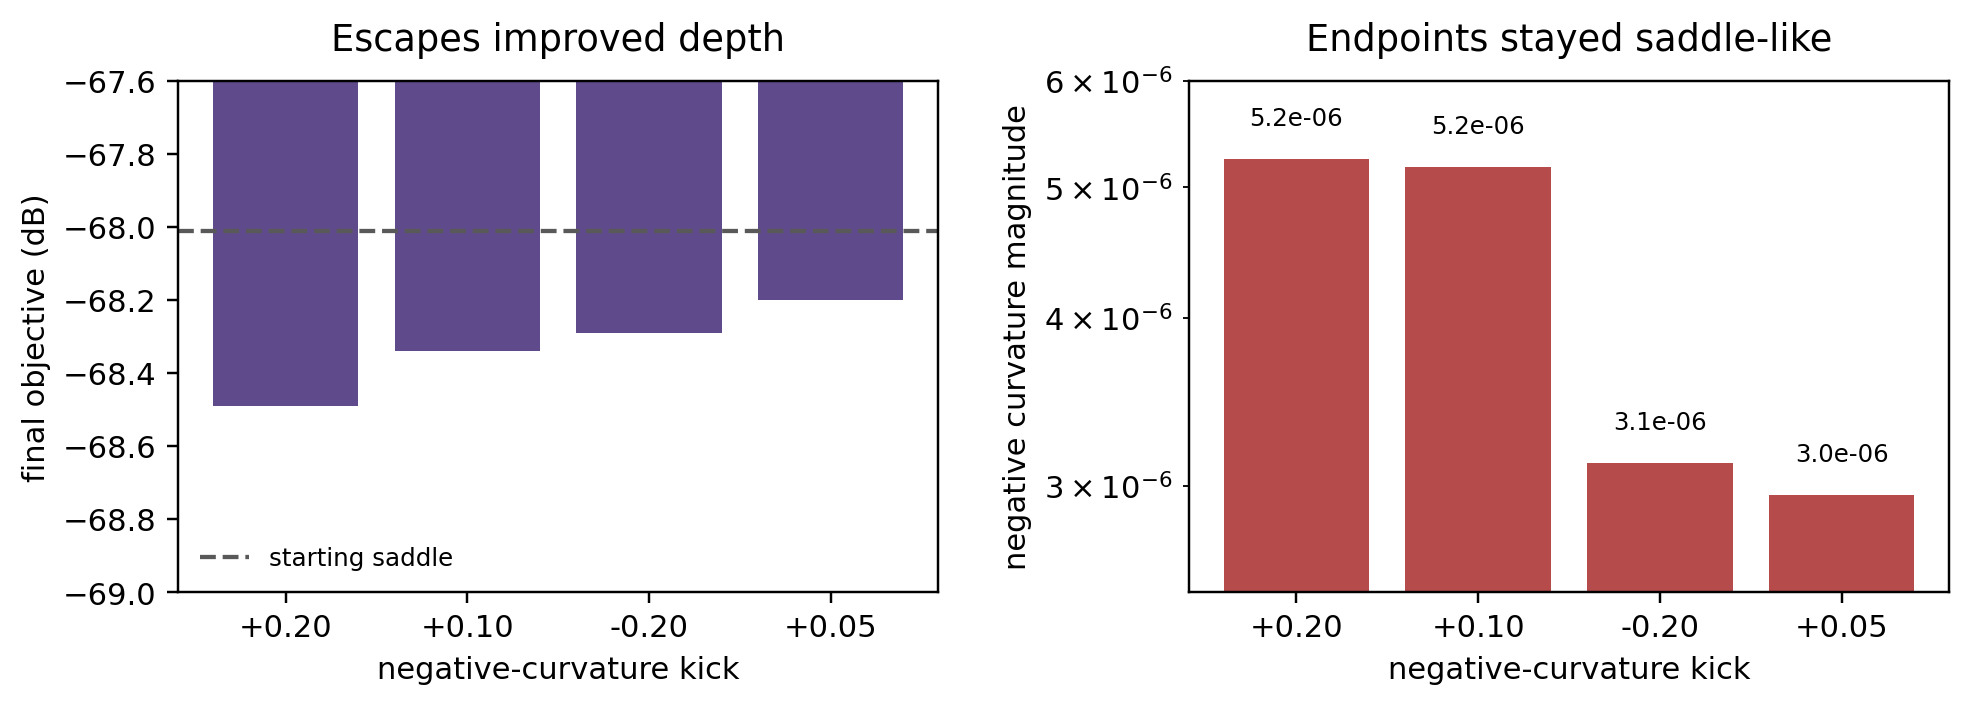
\includegraphics[width=0.90\linewidth]{figures/saddle_escape_summary_clean.png}
\caption{Negative-curvature escape from a competitive saddle. The escape steps
improved objective depth by roughly \(0.2\)--\(0.5\,\mathrm{dB}\), but all
tested endpoints remained saddle-like.}
\end{figure}

This is the practical optimization lesson: negative-curvature escape is useful,
but it should be described honestly. In the tested setting it found better
saddles, not clean minima.

\subsection*{Intuition Check}

If L-BFGS stops at a mountain pass, a Hessian eigenvector can tell us which way
the trail slopes down. But taking that trail does not guarantee we end in a
valley. We may just reach another mountain pass at a lower elevation.

\section{Implementation Surface}

\begin{center}
\small
\resizebox{\linewidth}{!}{%
\begin{tabular}{>{\raggedright\arraybackslash}p{0.30\linewidth}
                >{\raggedright\arraybackslash}p{0.62\linewidth}}
\toprule
\textbf{Component} & \textbf{Role} \\
\midrule
Recovery helpers & Grid sizing, gauge removal, forward validation, energy
drift, boundary checks, and standard-image saving. \\
Sweep recovery driver & Re-runs the simple-control ladder on repaired grids and
writes the retired-sweep summary. \\
Long-fiber validation reader & Pairs the scalar summary with the full saved
state so the actual phase can be revalidated. \\
Saddle diagnostic driver & Builds reduced-basis Hessians, classifies curvature,
and tests negative-curvature escape steps. \\
Standard-image helper & Writes the phase diagnostic and spectral-evolution
heat maps used in the result pages above. \\
\bottomrule
\end{tabular}}
\end{center}

The human-facing note avoids internal run labels. For reproduction, the local
README next to this PDF lists the relevant script families and result
summaries without making them part of the scientific narrative.

\section{What This Means For Future Work}

\textbf{Recovery first.} A candidate should not be promoted until the no-shaping
control, phase diagnostic, optimized heat map, unshaped heat map, edge
fraction, and energy drift have all been checked.

\textbf{Do not oversell achieved values.} If a run passes the physics checks
but does not converge, describe it as an achieved value or lower bound, not as
an optimum.

\textbf{Use saddle information operationally.} The Hessian should guide
restarts and continuation, not just decorate a report.

\textbf{Best next optimizer direction.} The evidence points toward
reduced-basis continuation plus a globalized second-order method: Newton-CG,
trust-region Newton, or cubic-regularized Newton with explicit
negative-curvature handling \cite{conn2000,nesterov2006,nocedal2006}.

\section{Presentation Capsule}

If this note becomes a validation slide, the clean message is:
\begin{itemize}
    \item Recovery work is how the project separates real saved results from numerically fragile or retired claims.
    \item A candidate is not promoted from a pretty heat map alone; it needs the control, phase diagnostic, edge/energy checks, and honest-grid rerun.
    \item Saddle diagnostics explain why reruns, perturbations, and restarts are scientifically necessary rather than bookkeeping.
    \item The safest story is not ``every old result was right.'' It is that the project now has a method for deciding which results survive.
\end{itemize}

\section{Limitations}

\textbf{The saddle ladder is one operating point.} The canonical SMF-28 result
is important, but not a proof that every fiber and power behaves the same way.

\textbf{The long-fiber result is not the long-fiber note.} It appears here only
because the recovery lane revalidated its saved state. A full long-fiber
interpretation belongs in a separate note after that lane stabilizes.

\textbf{No multimode claim is made here.} Multimode validation now belongs in
the separate multimode note. This recovery note only claims the single-mode
and long-fiber checks shown on its own pages.

\textbf{Images do not replace scalar gates.} The phase profiles and heat maps
are necessary for presentation, but the edge fraction and energy drift are what
make the pictures trustworthy.

\section{Reproduction Capsule}

For an existing candidate phase, the recovery checklist is:
\begin{enumerate}
    \item load the saved phase and its physical regime;
    \item remove constant and linear phase gauge over the active spectral band;
    \item choose a repaired time window from dispersion plus nonlinear
    broadening estimates;
    \item forward-propagate the flat pulse and candidate phase;
    \item require \(\eta_{\mathrm{edge}}<10^{-3}\) before trusting the result;
    \item rerun or re-anchor the optimization if the candidate survives;
    \item save the standard image set and visually inspect it.
\end{enumerate}

For saddle diagnostics, the checklist is:
\begin{enumerate}
    \item choose a reduced basis \(\phi=Bc\);
    \item compute the dense reduced Hessian at the candidate;
    \item classify the signs of the eigenvalues after ignoring gauge modes;
    \item if \(\lambda_{\min}<0\), try a small step along \(v_{\min}\);
    \item restart optimization and re-check the final Hessian class.
\end{enumerate}

\section{Sources and References}

\begin{thebibliography}{9}

\bibitem{agrawal2019}
G. P. Agrawal.
\textit{Nonlinear Fiber Optics}, 6th ed.
Academic Press, 2019.
\url{https://www.sciencedirect.com/book/9780128170427/nonlinear-fiber-optics}

\bibitem{hollenbeck2002}
D. Hollenbeck and C. D. Cantrell.
``Multiple-vibrational-mode model for fiber-optic Raman gain spectrum and
response function.''
\textit{Journal of the Optical Society of America B}, 19(12), 2886--2892, 2002.
\url{https://doi.org/10.1364/JOSAB.19.002886}

\bibitem{hult2007}
J. Hult.
``A fourth-order Runge-Kutta in the interaction picture method for simulating
supercontinuum generation in optical fibers.''
\textit{Journal of Lightwave Technology}, 25(12), 3770--3775, 2007.
\url{https://doi.org/10.1109/JLT.2007.909373}

\bibitem{nocedal2006}
J. Nocedal and S. J. Wright.
\textit{Numerical Optimization}, 2nd ed.
Springer, 2006.
\url{https://doi.org/10.1007/978-0-387-40065-5}

\bibitem{liu1989}
D. C. Liu and J. Nocedal.
``On the limited memory BFGS method for large scale optimization.''
\textit{Mathematical Programming}, 45, 503--528, 1989.
\url{https://doi.org/10.1007/BF01589116}

\bibitem{conn2000}
A. R. Conn, N. I. M. Gould, and P. L. Toint.
\textit{Trust Region Methods}.
SIAM, 2000.
\url{https://doi.org/10.1137/1.9780898719857}

\bibitem{nesterov2006}
Y. Nesterov and B. T. Polyak.
``Cubic regularization of Newton method and its global performance.''
\textit{Mathematical Programming}, 108, 177--205, 2006.
\url{https://doi.org/10.1007/s10107-006-0706-8}

\bibitem{dauphin2014}
Y. N. Dauphin, R. Pascanu, C. Gulcehre, K. Cho, S. Ganguli, and Y. Bengio.
``Identifying and attacking the saddle point problem in high-dimensional
non-convex optimization.''
NeurIPS, 2014.
\url{https://arxiv.org/abs/1406.2572}

\end{thebibliography}

\end{document}
